%\documentclass[printmode,oneside,pl]{mgr}  % do publikacji elektronicznej
\documentclass[printmode,pl]{mgr}  % do wydruku dwustronnego
%\documentclass[printmode,pl,draft]{mgr}  % do wydruku dwustronnego w~wersji roboczej
%\documentclass[printmode,en]{mgr}  % do wydruku dwustronnego ze stroną tytułową w~wersji angielskiej

%----------------------| Wybór strony kodowej |------------------------

\usepackage[utf8]{inputenc}

%-------------------------| Wybór kroju pisma |------------------------

%% Najpierw (chyba) należy wybrać czcionkę tekstu, potem matematyki

%% wybór czcionki Computer Concrete specjalnie zaprojektowanej do użycia 
%% z~czcionką matematyczną euler (nie ma ona niestety wersji bold - proponuje się więc użycie bolda z kroju
%%   Computer Modern Sans Serif)
%\usepackage{beton}             % ZALECANA DO SKŁADU TEKSTÓW PO ANGIELSKU
%\renewcommand{\bfdefault}{sbc} % to use Computer Modern Sans Serif demibold condensed fonts as bold 
%% choć może komuś bardziej podobać się będzie ten krój normalnej szerokości 
%\renewcommand{\bfdefault}{sb} % to use Computer Modern Sans Serif demibold fonts as bold 

%% alternatywny wybór Antykwy Półtawskiego - czcionki zaprojektowanej
%% specjalnie dla języka polskiego uwzględniającej jego rytm 
%\usepackage{antpolt}
%% alternatywny wybór Antykwy Toruńskiej - bardziej "współczesnej",
%% całkowicie polskiej czcionki
\usepackage{anttor}             % ZALECANA DO SKŁADU TEKSTÓW PO POLSKU
%\usepackage[math]{anttor}      % math włącza antykwę także w~matematyce
                                % ale chyba coś psuje :( (np. brak strzałek)

%% alternatywnie wybór czcionki URW Palladio
%\usepackage{newpxtext}  % Palatino font
%\linespread{1.05}  % Palatino needs more leading space (between lines)

%% ustawienie czcionki eulerowskiej do składu wyrażeń matematycznych
%\usepackage[euler-digits,small]{eulervm}
\usepackage{eulervm}

%% ustawienie czcionki bezszeryfowej Monospace (typewriter, code) font (last) - skład poleceń, wydruków programów
\usepackage[varqu,varl]{inconsolata}

%-------------------------| Sprawy polskie |------------------------

\usepackage[T1]{fontenc} % bez tego są złe znaki / { } w czcionce tt
                         % ale musi być użyty pakiet polski bez opcji
                         % wybierającej układ - gdy zamarkowane
                         % używamy pakiet polski z~opcją wyboru układu
\usepackage{polski}
%\usepackage[OT4]{polski} % domyślnie?

%---------------------------| Pakietologia |-------------------------

\usepackage{geometry}           % manipulowanie geometrią łamu
\usepackage{indentfirst}        % wcięcia akapitowe w pierwszych paragrafach rozdziałów
\usepackage[dvipsnames]{xcolor} % by mieć nazwy kolorów w~rodzaju \green

%% zmiana formatowania tytulariów
%\usepackage[raggedleft]{titlesec}

\usepackage[titles]{tocloft}    % do formatowania spisów

%% modyfikacja odstępów między pozycjami w spisie treści
%% w razie potrzeby zmieniamy nieco odstępy przed rozdziałami i podrozdziałami w spisie
%% treści by uniknąć pojedynczego samotnego tytułu rozdziału/podrozdziału na dole/górze strony
%% i by ładnie się zmieściła notka o latechu
\addtolength{\cftbeforechapskip}{-1.3ex}
\addtolength{\cftbeforesecskip}{0.02ex}
 
%% %%% Bibliography %%%%%%%%%%%%%%%%%%%%%%%%%%%%%%%%%%%%%%%%%%%%%%%%%%%%%%%%%%%%%%%
%% \usepackage{xpatch}  % ?recommended for biblatex?
%% \usepackage[% biblatex has more styles, etc. than the default natbib
%%     backend=bibtex,  % by default it's biber,
%%                      % they say that biber is better but it didn't work for me
%%     citestyle=numeric-comp,  % cite by number, will collapse ranges, e.g. [3-6]
%%     bibstyle=numeric,  % printbibliography will show as [1], [2], ...
%%     giveninits=true  % use given/first names initials only, e.g. "K. Tchoń"
%% ]{biblatex}
%% % names bibtex, biber, biblatex and natbib are quite confusing, see:
%% % https://tex.stackexchange.com/questions/25701/bibtex-vs-biber-and-biblatex-vs-natbib


%%modyfikacja odstępów między pozycjami w bibliografii
\let\oldbibliography\thebibliography
\renewcommand{\thebibliography}[1]{%
  \oldbibliography{#1}%
  \setlength{\itemsep}{0pt plus 0.3ex}%
}

%% ustawienie maksymalnej liczby i obszaru dla obiektów pływających (rysunków, tabel)
\setcounter{topnumber}{3}
\setcounter{totalnumber}{4}
\renewcommand{\topfraction}{.8}

\usepackage{graphicx}                % dołaczanie i manipulowanie grafikami
\usepackage[export]{adjustbox}       % więcej komend operujących na "pudełkach"
\usepackage[caption = false]{subfig} % obsługa rysunków z częściami

%\usepackage{svg}                % dołączanie grafik w formacie svg
\usepackage[inkscapepath=svgdir]{svg}  % w nowszych wersjach

\usepackage{tikz}               % dołączanie grafik w formacie TikZ
\usepackage{makecell}           % trochę tikzowej magii
    \tikzstyle{block} = [draw, fill=blue!20, rectangle, 
     minimum height=3em, minimum width=6em]
    \tikzstyle{sum} = [draw, fill=blue!20, circle, node distance=3.5cm]
    \tikzstyle{input} = [coordinate]
    \tikzstyle{output} = [coordinate]
    \tikzstyle{pinstyle} = [pin edge={to-,thin,black}]    
    \usetikzlibrary{arrows,automata,calc,positioning}
\usepackage{standalone}  

\usepackage{pgfplots}           % do robienia wykresów 
\pgfplotsset{compat=1.5}        %% why 1.5? pl. update

\usepackage{mathtools}          % doskonałe pakiety rozszerzające do matematyki
\usepackage{amssymb, amsfonts}  % mathtools zastępuje amsmath (naprawione błedy, dodane rozszerzenia) 
\usepackage{wasysym}            % trochę więcej różnych symboli (buźki)
%\usepackage[fleqn]{mathtools}  % równania w wersji dosuniętej w lewo
%% automatyczne numerowanie jedynie tych równań, do których są odwołania w~tekście
%\mathtoolsset{showonlyrefs=true}

%% symbole do oznaczania stopek w~miejsce liczb
\renewcommand{\thefootnote}{\fnsymbol{footnote}}
%% powtórzone z latex.ltx - w przeciwnym razie znika symbol \textbardbl przy
%% wybranej Antykwie Toruńskiej (sprawdzić co z innymi definicjami z omsenc.def,
%% sprawdzić czy też przy innych czcionkach)
\DeclareTextSymbolDefault{\textbardbl}{OMS}
%% automatyczne resetowanie wartości licznika stopek użyteczne przy użyciu symboli
%% do oznaczania stopek w~miejsce liczb (liczba dostępnych symboli wynosi tylko 9)
\usepackage{etoolbox,pdftexcmds}
\makeatletter
\patchcmd{\footnote}
  {\stepcounter\@mpfn}
%  {\stepcounter\@mpfn\check@overflow\@mpfn} %%było w~przykładzie
  {\stepcounter\@mpfn\check@overflow}
  {}{}
\newcommand{\check@overflow}{%
  \ifnum\pdf@strcmp{\@mpfn}{footnote}=\z@
    \ifnum\value{footnote}>9  %
      \setcounter{footnote}{1}%
    \fi
  \fi
}
\makeatother

\usepackage{hyperref}           % obsługa aktywnych odnośników i hypertekstu
\usepackage{url}                % obsługa adresów url

%% pakiet minted do wydruków programów
%% 'minted' gives much better highlight then the default listings,
%% but it reqires Python with Pygments (check the documentation of minted)
%% it also requires passing '-shell-escape' option to pdflatex during compilation
\usepackage[%
  cache=false,
  chapter,
  %    outputdir=build,  % if building in separate directory, this must be included
                         % ale nie zawsze działa poprawnie :( 
    newfloat  % required if multi-page floating listings are needed (see below)
]{minted}  % (note: from my experience must be loaded before 'csquotes')
%% by wybrać inny styl - lista dostępnych styli: pygmentize -L styles
%\usemintedstyle{igor}
\SetupFloatingEnvironment{listing}{name=Wydruk}
%% kolor tła używany w~wydrukach
\definecolor{OurListingBackground}{rgb}{0.95,0.95,0.95}
%% fix the minted@colorbg environment bug
\makeatletter
\renewenvironment{minted@colorbg}[1]
 {\def\minted@bgcol{#1}%
  \noindent
  \begin{lrbox}{\minted@bgbox}
  \begin{minipage}{\linewidth-2\fboxsep}}
 {\end{minipage}%
  \end{lrbox}%
  \setlength{\topsep}{\bigskipamount}% set the vertical space
  \trivlist\item\relax % ensure going to a new line
  \colorbox{\minted@bgcol}{\usebox{\minted@bgbox}}%
  \endtrivlist % close the trivlist
 }
\makeatother
%% koniec ustawień pakietu minted

%\usepackage{csquotes}

%%pakiet do robienia notatek w trakcie pracy
\usepackage[textsize=footnotesize]{todonotes}
\makeatletter   %spolszczenie
\renewcommand{\@todonotes@todolistname}{Do zrobienia}
\renewcommand{\@todonotes@MissingFigureText}{Rysunek}
\renewcommand{\@todonotes@MissingFigureUp}{{\small Brakujący}}
\renewcommand{\@todonotes@MissingFigureDown}{{\small rysunek}}
\makeatother

%% dodaje w pliku wynikowym klucze etykiet i referencji - wygodne przy pracy nad tekstem
%\usepackage{showkeys}

%%inne przydatne
%\usepackage{fancyhdr}
%\usepackage{fancyvrb}
%\usepackage{lipsum}  
%\usepackage{listings}  %% alternatywa do używanego tutaj pakietu minted 

%-----------------------| End of pakietologia |----------------------

%---------------------------| Tytularia |---------------------------

% Zmień dane stosownie do tytułu i autora pracy tutaj
% ALE TEŻ I W POLECENIU \pdftitle NIECO PONIŻEJ! (Hyper data general configuration)
\author{Roberto Orozco\\{\color{red}Robert Muszyński\\\footnotesize (kompilacja \today)}}
\title{Bąk jaki jest każdy widzi. Studium zachowań\\{\em\color{red} Przykład
    i~wytyczne formatowania\\ pracy dyplomowej}}
\engtitle{Top is a top. Case study}
\supervisor{Dr inż. Robert Muszyński,\\ Katedra Cybernetyki i~Robotyki}
\field{Automatyka i~Robotyka (AIR)}
\specialisation{Robotyka (ARR)}
\date{2022}

%-------------------------| Hyper data general configuration |------------------------

\hypersetup{unicode,
                          % DANE DOKUMENTACJI
   pdfauthor={Roberto Orozco, Robert Muszyński},
   pdftitle={Bąk jaki jest każdy widzi. Studium zachowań - Przykład
    i~wytyczne formatowania pracy dyplomowej},
   pdfsubject={Praca dyplomowa inżynierska - przykład i~wytyczne},
   pdfkeywords={bąk, Lagrange top, Euler top, praca dyplomowa, formatowanie, wytyczne},
                          % USTAWIENIA DOKUMENTU
   pdfpagemode=UseOutlines,   % otwiera dokument w trybie jednej strony
   pdfpagelayout=SinglePage,  %
   pdfstartview={Fit},        %
   pdfstartpage=1,            % na podanej stronie
   bookmarksopen=true,        % rozwinięcie zakładek
   bookmarksopenlevel=1,      % do jakiego poziomu
   colorlinks=true,       % kolorowanie odnośników zamiast ramki wokół nich
   breaklinks,            %
   citecolor=cyan,        % kolor odnośników do bibliografii, domyślnie zielony
   filecolor=red,         % kolor odnośników do lokalnych plików, domyśnie magenta
   linkcolor=blue,        % kolor odnośników wewnętrznych, domyślnie czerwony
   menucolor=green,       % kolor pozycji menu Acrobata, domyślnie czerwony
   urlcolor=blue          % kolor odnośników do adresów internetowych, domyślnie cyan
}

%-------------------------| Geometria strony |-----------------------------

\geometry{
    top = 25mm,
    headheight = 15mm,
    headsep = 3mm,
    textheight = 24cm,
    textwidth = 16cm,
    marginparwidth = 25mm
}

%---------------------| Często używane polecenia |-------------------

\newcommand{\red}{\color{red}}
\def\BibTeX{{\rm B\kern-.05em{\sc i\kern-.025em b}\kern-.08em
    T\kern-.1667em\lower.7ex\hbox{E}\kern-.125emX}}

\newtheorem{uwaga}{Uwaga}
\newtheorem{twr}{Twierdzenie}
%------------------------------------| END |-------------------------------------

%----------------------------| Definicje symboli matematycznych |-------------------------

\newcommand{\angmom}{\boldsymbol{m}}
\newcommand{\bdvelo}{\boldsymbol{\omega}_B}
\newcommand{\grav}{\boldsymbol{g}}
\newcommand{\lagran}{L(\boldsymbol{q},\boldsymbol{\dot{q}})}
\newcommand{\COMvec}{\boldsymbol{r}_B}
\newcommand{\ee}{\boldsymbol{e}}
\newcommand{\FF}{\boldsymbol{F}}
\newcommand{\xx}{\boldsymbol{x}}
\newcommand{\qq}{\boldsymbol{q}}
\newcommand{\RR}{\boldsymbol{R}}
\newcommand{\TT}{\boldsymbol{T}}
\newcommand{\pp}{\boldsymbol{p}}
\newcommand{\iner}{\boldsymbol{I}_B}
\newcommand{\vv}{\boldsymbol{v}}
\newcommand{\bbs}{\boldsymbol}
\DeclareMathOperator{\const}{const}
\DeclareMathOperator*{\rank}{rank}  %star changes sub- and superscripts placement
%------------------------------------| END |-------------------------------------

%--------------------------| Ścieżki do rysunków |-------------------------------

\graphicspath{{./figures/chapter_01/}{./figures/chapter_02/}{./figures/chapter_03/}{./figures/chapter_04/}}

%--------| kontrola dołączanych plików - wygodne przy pracy nad tekstem |--------

%\includeonly{sources/Od_Autora,sources/02_czym_jest_bak}

%-------------------------| The document starts here |-------------------------------
\begin{document}

\pdfbookmark{Strona tytułowa}{tytul}
\maketitle
%% informacja o sposobie udostępniania tego dokumentu
\thispagestyle{empty}
\mbox{}
\vfill

\noindent
{\bf Robert Muszyński, Roberto Orozco}\\
{\bf Wrocław 2022}\\[2ex]
  
\includegraphics[width=0.18\textwidth]{figures/CC-BY-SA_icon_svg.png}\hfill
\begin{minipage}[b]{0.79\textwidth}
 \small Szablon jest dostępny na licencji Creative Commons: \emph{Uznanie au\-tor\-stwa-Na tych samych warunkach 4.0 Polska}
\end{minipage}\vspace{2ex}

\noindent
{\normalsize Utwór udostępniany na licencji Creative Commons: uznanie
  autorstwa, na tych samych warunkach. Udziela się zezwolenia do
  kopiowania, rozpowszechniania i/lub modyfikacji treści utworu
  zgodnie z zasadami w/w licencji opublikowanej przez Creative
  Commons. Licencja wymaga podania oryginalnego autora utworu, a
  dystrybucja materiałów pochodnych może odbywać się tylko na tych
  samych warunkach (nie można zastrzec, w jakikolwiek sposób
  ograniczyć, ani rozszerzyć praw do nich). Tekst licencji jest
  dostępny pod
  adresem: \url{https://creativecommons.org/licenses/by-sa/4.0/legalcode.pl}. Podczas
  redakcji pracy dyplomowej notkę tę można usunąć, licencja dotyczy
  bowiem zredagowanego opisu, a nie samego latechowego
  szablonu.  Szablon można wykorzystywać bez wzmiankowania o
  jego autorze.}


%% dedykacja
%%\dedication{6cm}{To jest przykładowa treść opcjonalnej dedykacji,
%%  należy ją zmienić lub usunąć w całości polecenie
%%  \texttt{\textbackslash dedication}}

\cleardoublepage
\pdfbookmark{\contentsname}{Contents}
\tableofcontents            %spis treści
\markboth{\contentsname}{\contentsname}
%\newpage
%\thispagestyle{empty}
%\cleardoublepage
%\thispagestyle{plain}

\mbox{}\vfill\hfill
\begin{minipage}{0.5\linewidth} 
  {\tiny \noindent Do składu pracy wykorzystano system przygotowania
    dokumentów~\LaTeX, opracowany przez
    L.~Lamporta\index{latex>\LaTeX} [Lam94], będący nakładką
    systemu \TeX, [Knu86a,Knu86b].  Matematyczne czcionki o nazwie
    {AMS Euler}, których używamy w tej pracy, zostały przygotowane
    przez H.\ Zapfa [KZ86], przy współpracy z~D.\ Knuthem i~jego
    studentami, na zlecenie Amerykańskiego Towarzystwa Matematycznego.
    %% Przy wybranej Antykwie Toruńskiej/Półtawskiego odznacz odpowiednio poniższe
    Wybrane czcionki składu tekstu, Antykwa Toruńska [Now97] -- jeden
    %Wybrane czcionki składu tekstu, Antykwa Półtawskiego [Now99] -- jeden
    z~nielicznych krojów pisma zaprojektowany specjalnie dla języka
    polskiego w~sposób uwzględniający jego rytm -- w~odczuciu autora
    doskonale współgrają z~kształtem czcionki {AMS Euler}, pozwalając
    na uzyskanie harmonijnej całości.
    % %% Przy wybranych czcionkach Concrete odznacz poniższe
    % Czcionki składu tekstu, zwane {Concrete Roman} i {Concrete
    %   Italic}, należące do knuthowskiej rodziny czcionek {Computer
    %   Modern}, zostały specjalnie przystosowane do kształtu czcionki
    % {AMS Euler} na potrzeby książki [GKP96].
    % %% Przy wybranych czcionkach URW Palladio odznacz poniższe
    % Czcionka składu tekstu, zwana URW Palladio jest klonem zapfoskiej rodziny
    % czcionek o~nazwie Palatino [LPn05] i~zdaniem autora świetnie współgra
    % z~kształtem czcionki {AMS Euler}.
    Składu bezszeryfowego tekstu maszynowego dokonano z~użyciem
    opracowanej przez R. Leviena czcionki o~nazwie Inconsolata
    [Lev15]\footnote{\red\tiny Chyba warto takie informacje szerzyć}.


\vspace{-4mm}

 \makeatletter
\renewenvironment{thebibliography}[1]
     {%
        \tiny%
      \list{\@biblabel{\@arabic\c@enumiv}}%
           {\settowidth\labelwidth{\@biblabel{#1}}%
\setlength{\itemsep}{2.5mm}
            \leftmargin\labelwidth
            \advance\leftmargin\labelsep
            \@openbib@code
            \usecounter{enumiv}%
            \let\p@enumiv\@empty
            \renewcommand\theenumiv{\@arabic\c@enumiv}}%
      \sloppy\clubpenalty4000\widowpenalty4000%
      \sfcode`\.\@m\vspace{5mm}}
     {\def\@noitemerr
       {\@latex@warning{Empty `thebibliography' environment}}%
      \endlist}

\makeatother

\begin{thebibliography}{Knu86b}

% %% Odmarkować pozycję gdy wybrane czcionki Concrete
% \bibitem[GKP96]{GKP96loc}
% R.~L. Graham, D.~E. Knuth i O.~Patashnik,
% \newblock { Matematyka konkretna}.
% \newblock PWN, Warszawa, 1996.\vspace{-3mm}

\bibitem[Knu86a]{Knuth86loc}
D.~E. Knuth,
\newblock { The \TeX book, volume {A} of Computers and Typesetting}.
\newblock Addison-Wesley, Reading, 1986.\vspace{-3mm}

\bibitem[Knu86b]{Knuth86aloc}
D.~E. Knuth,
\newblock { \TeX: {The} Program, volume {B} of Computers and Typesetting}.
\newblock Addison-Wesley, Reading, 1986.\vspace{-3mm}

\bibitem[KZ86]{KnZa89loc}
D.~E. Knuth i H.~Zapf,
\newblock {AMS} {Euler} --- {A} new typeface for mathematics.
\newblock { Scholary Publishing}, {20}:131--157, 1986.\vspace{-3mm}

\bibitem[Lam94]{Lamport94loc}
L.~Lamport,
\newblock { \LaTeX: A Document Preparation System}.
\newblock Addison-\mbox{-Wesley}, Reading, 1994.\vspace{-3mm}

\bibitem[Lev15]{Levien15loc}
R.~Levien,
\newblock {Inconsolata}.
\newblock \url{https://levien.com/type/myfonts/inconsolata.html}, 2015.\vspace{-3mm}

% %% Odmarkować pozycję przy wybranej czcionce URW Palladio
% \bibitem[LPn05]{LinotypePalatino05loc}
% Linotype Palatino nova: A classical typeface redesigned by Hermann Zapf,
% \newblock Linotype Library GmbH, 2005.\vspace{-2mm}

%% Odmarkować pozycję przy wybranej Antykwie Toruńskiej
\bibitem[Now97]{nowacki97loc}
J.~Nowacki,
\newblock {Antykwa} {Toruńska} -– od początku do końca polska czcionka.
\newblock {\em Biuletyn Polskiej Grupy Użytkowników Systemu \TeX}, 9:26--27,
  \nolinebreak1997.\vspace{-2mm}

% %% Odmarkować pozycję przy wybranej Antykwie Półtawskiego
% \bibitem[Now99]{nowacki99}
% J.~Nowacki,
% \newblock Piórkiem i {MetaPost-em}, czyli {Antykwa} {Półtawskiego}.
% \newblock {\em Biuletyn Polskiej Grupy Użytkowników Systemu \TeX}, 12:49--53,
%   \nolinebreak1999.\vspace{-2mm}

\end{thebibliography}
}
\end{minipage}
       %notka o systemie składu i czcionkach
%% Side note about LaTeX and the fonts being used in the thesis
\mbox{}\vfill\hfill
\begin{minipage}{0.618033988749895\textwidth}
    \begin{refsection}[font-note-literature.bib] % separate bibliography for this minipage
                                                 % this resource was added with \addsectionbib
        {% smaller font for paragraph and bibliography
            \scriptsize%
            \renewcommand*{\bibfont}{\scriptsize}%
            \noindent%
            %
            For typesetting this thesis,
            the~\LaTeX{} document preparation system has been used.
            \LaTeX{} has been developed by L.~Lamport~\cite{lamport:latex},
            and~is an~overlay on top of the~\TeX{} system~\cite{knuth:texbook}.
            %
            Mathematical fonts called AMS~Euler which have been used in~this document,
            have been commissioned by the American Mathematical Society
            and~designed by H.\ Zapf~\cite{zapf:ams-euler} with the assistance of D.\ Knuth and his students.
            %
            The~URW~Palladio font, used for roman text,
            is a~clone of H.\ Zapf's old-style typeface called Palatino~\cite{zapf:palatino}.
            %
            Typesetting of sans-serif monospaced text has been done using
            Inconsolata font, created by R.\ Levien~\cite{levien:inconsolata}.
            %
            \noindent
            \printbibliography[heading=none,locallabelwidth=true] % print section bibliography
        }
    \end{refsection}
\end{minipage}
   %przykładowa wersja angielska notki - używa pakietu biblatex

%---------------------------| Część właściwa dokumentu |---------------------------

\chapter*{Od Autorów}
\addcontentsline{toc}{chapter}{Od Autorów}
\markboth{Od Autorów}{Od Autorów}

Niniejszy przykład przygotowano celem ułatwienia opracowania prac dyplomowych z~wykorzystaniem dostarczonego przez Adama Ratajczaka stylu \texttt{mgr} systemu \LaTeX{}. Styl \texttt{mgr} służy do przygotowywania prac dyplomowych na Wydziale Elektroniki, Fotoniki i~Mikrosystemów oraz Wydziale Informatyki i~Telekomunikacji Politechniki Wrocławskiej i~jego głównym zadaniem jest odpowiednie sformatowanie strony tytułowej dokumentu\footnote{W razie potrzeby plik z~opisem klasy \texttt{mgr} można znaleźć na stronie autora \cite{Ratajczak}; tam też można znaleźć dokument szczegółowo opisujący sposób korzystania z~klasy \texttt{mgr} (\texttt{manual.pdf}) -- prezentowany tu przykład zawiera już najnowszą wersję pliku ze stylem \texttt{mgr}.}. Aktualną wersję prezentowanego przykładu można znaleźć na stronie internetowej \cite{wzor_praca} w~części ,,Inne materiały''\footnote{Informacje o~zauważonych błędach/brakach prosimy kierować na adres \texttt{mucha@pwr.edu.pl}.}. Więcej porad technicznych dotyczących składu pracy dyplomowej można znaleźć w~szablonie przygotowanym przez Tomasza Kubika \cite{kubik}. Listę zmian pozwalających przekształcić ten przykładowy dokument w~swoją własną pracę dyplomową zebrano w~podrozdziale~\ref{sec:listakontrolna}.

Dostarczony zestaw plików zawiera docelowy plik wzorcowy dokumentu z~pracą dyplomową w~formacie PDF \texttt{praca\_dyplomowa\_wzor.pdf} (który pewnie właśnie czytasz) oraz archiwum \texttt{praca\_dyplomowa\_wzor.zip}\footnote{Po jego rozpakowaniu otrzymujemy katalog \texttt{praca\_dyplomowa\_wzor} z~wszystkimi niezbędnymi do pracy plikami -- w~tym katalogu przeprowadzamy opisaną poniżej kompilację. By edytować dokument w~systemie Overleaf wystarczy wczytać do niego nierozpakowane archiwum (\texttt{New Project} $\rightarrow$ \texttt{Upload Project}).} zawierające zestaw jego plików źródłowych: plik główny \texttt{main.tex}\footnote{Pliki źródłowe przygotowano z~zastosowaniem systemu kodowania znaków UTF8 i~windowsowymi znakami nowej linii (CRLF). Konwersja znaków nowej linii do formatu uniksowgo (zazwyczaj niepotrzebna): \texttt{dos2unix plik\_we plik\_wy} lub \texttt{tr -d '\textbackslash r' < plik\_we > plik\_wy}.}, pliki z~treścią rozdziałów (znajdujące się w~katalogu \texttt{sources}), pliki rysunków (katalog \texttt{figures}). By skompilować dostarczone źródła do postaci wynikowej należy użyć kompilatora \LaTeX{}a oraz \BibTeX{}a w~sekwencji\footnote{Zakładamy tu, że wykorzystywana jest lokalna instalacja \LaTeX{}a z~poziomu powłoki tekstowej (np. \texttt{bash}). Takie rozwiązanie pozwala na pracę bez dostępu do internetu, jest bardzo szybkie i~daje się łatwo ,,automatyzować'' wedle potrzeby -- przez użycie skryptów powłoki, uruchamianie procesu kompilacji z~poziomu używanego edytora (np. emacsa:), integrację z~lokalną ,,wyświetlarką pdfów''. Warto spróbować! Przy korzystaniu z~innych rozwiązań, jak te wymienione w~podrozdziale~\ref{narzedzia}, należy zadbać, by w~ich ramach została wykonana odpowiednia sekwencja poleceń w~celu uzyskania aktualnego, wynikowego pliku PDF.}\footnote{W~niektórych systemach może potrzebne być użycie opcji pdflatecha \texttt{--shell-escape}.}\vspace{-3mm}
\begin{verbatim}
  pdflatex main
  bibtex main
  pdflatex main
  pdflatex main
\end{verbatim}
Bezbłędny przebieg wykonania powyższych poleceń wyprodukuje plik \texttt{main.pdf}, który powinien wyglądać identycznie jak ten wzorzec, co równocześnie potwierdzi poprawność i~kompletność wykorzystywanej instancji systemu \LaTeX. Dokument można kompilować we fragmentach z~zachowaniem poprawności wszystkich odwołań używając w~jego preambule polecenie \texttt{\textbackslash includeonly} z~podaną listą plików rozdziałów do dołączenia\footnote{Przykład użycia zamieszczono w~pliku \texttt{main.tex}.}.

W~tym przykładzie zdecydowano się na wykorzystanie do składu tekstu kroju pisma zaprojektowanego specjalnie dla języka polskiego o~nazwie Antykwa Toruńska \cite{antykwa,antykwab} wraz matematyczną czcionką o~nazwie AMS Euler \cite{eulerfont}, o~czym napisano w~dodanej pod spisem treści notce. Domyślne kroje pisma można łatwo przywrócić usuwając odpowiednie pakiety z~preambuły dokumentu\footnote{W preambule pokazano także, w~jaki sposób można włączyć inne kroje -- zwracamy uwagę, szczególnie osób piszących prace po angielsku, na kroje o~nazwach Computer Concrete oraz URW Palladio (pierwszy będący odmianą kroju Concrete Roman, zaś drugi kroju Palatino) \cite{concr, palla, antyk}.}. 

Prezentowany dokument, oprócz wskazania sposobu wykorzystania stylu \texttt{mgr}, opisuje podstawowe zasady tworzenia pracy dyplomowej. Jednakże należy podkreślić, że intencją autorów nie jest dostarczenie jeszcze jednego dokumentu traktującego o~metodach formatowania tekstu w~środowisku \LaTeX, ale zilustrowanie w~jednym miejscu sposobów uzyskania podstawowych elementów występujących w~typowej pracy dyplomowej\footnote{Dziś częstokroć dany efekt można uzyskać w~\LaTeX{}u na kilka sposobów i~wybór/znalezienie tego ,,najlepszego/właściwego'' może zająć sporo czasu. Stąd pomysł, by w~tym dokumencie podzielić się ,,doświadczeniem'' zdobytym przez wcześniejsze ,,pokolenia dyplomantów''. Jeśli masz więc jakieś uwagi śmiało pisz na \texttt{mucha@pwr.edu.pl}.}. Zamysł całości jest taki: Znajdź w~dostarczonym pdfie element, którego potrzebujesz i~zobacz w~jego źródłach, w~jaki sposób został uzyskany.

W~kolejnych rozdziałach tekst zapisany kolorem czerwonym stanowi komentarz do przytoczonych fragmentów pracy autorstwa Roberto Orozco \cite{roberto}, zwracający uwagę na rzeczy, które te fragmenty ilustrują. Komentarz każdorazowo dotyczy tekstu go poprzedzającego. W~źródle dokumentu można zobaczyć jak dany efekt uzyskano. A~poniżej zebrano podstawowe wytyczne dotyczące redakcji tekstu. Więcej o~zasadach użycia systemu \LaTeX{} można poczytać w~,,Nie za krótkim wprowadzeniu\ldots'' \cite{lshort2e} oraz szerzej w~,,Książce kucharskiej\ldots'' \cite{latex_kucharska}. Łagodne wprowadzenie do \LaTeX{}a zapewnia także kurs w~pdfie \cite{lshortpie}, kurs w~htmlu \cite{latex_kurs}, czy dokumentacja środowiska Overleaf \cite{latex_overleaf}. W~razie czego warto też zajrzeć na stronę Wikibooks \cite{latex_wiki2}.

Autorzy są wdzięczni Jędrzejowi Boczarowi, dyplomantowi specjalności Embedded Robotics w~roku 2019, za uprzejmą współpracę i~recenzję całości \cite{jedrzej}.

\section{Narzędzia}
\label{narzedzia}

\begin{enumerate}
%\setlength{\itemsep}{0pt}
\item \LaTeX{} jest językiem znaczników do formatowania dokumentów tekstowych, także zawierających elementy graficzne, który dostarcza zestawu makr stanowiących nadbudowę dla systemu składu \TeX, \cite{latex, latex_wiki, latex_wiki2}. Podstawowym oprogramowaniem służącym do kompilacji dokumentów opisanych w~tym języku jest system \LaTeX\footnote{który korzystając z~systemu \TeX{} na podstawie plików źródłowych produkuje plik wynikowy w~formacie \texttt{DVI} (\emph{ang. device independent}) stanowiący bazę do uzyskania innych formatów jak PDF czy PS \cite{dvi_wiki}}. Jednakże ponieważ obecnie dostępnych jest kilka alternatywnych dla \TeX{}a narzędzi, takich jak pdf\TeX, Xe\TeX{} czy Lua\TeX, towarzyszą im dedykowane systemy kompilacji jak pdf\LaTeX{} czy Xe\LaTeX. Autorzy tego dokumentu do jego kompilacji wykorzystali system pdf\LaTeX\footnote{który na podstawie plików źródłowych produkuje bezpośrednio plik wynikowy w~formacie PDF}, zaś zainteresowanych ,,innymi smakami \TeX{}a'' odsyłają do takich pozycji jak \cite{latex_kucharska,tex_legacy,xxxtex}.
  
\item Ponieważ sam \LaTeX{} jest systemem składu tekstu wyposażonym jedynie w~interfejs wiersza poleceń (\emph{ang. command-line interface})\footnote{nazywany przez niektórych interfejsem linii komend}, do pracy z~nim potrzebny jest edytor tekstowy, który pozwoli wprowadzić pożądaną treść do komputera. Wygodnie jest korzystać w~tym celu z~któregoś z~edytorów dostosowanych do składni \LaTeX{}a\footnote{Ale oczywiście możliwe jest użycie dowolnego edytora tekstu, byle tylko pozwalał on na zapisywanie plików w~wybranej do pracy stronie kodowej.}. W~przypadku przynajmniej podstawowej znajomości składni \LaTeX{}a na wygodną pracę pozwoli odpowiednio skonfigurowany edytor ogólnego przeznaczenia, jak chociażby GNU Emacs\footnote{W celu ułatwienia konfiguracji emacsa do tego opisu dołączony jest przykładowy plik konfiguracyjny \texttt{emacs\_conf}. Jego zawartość w~miarę potrzeby należy dodać do lokalnego pliku konfiguracyjnego emacsa (\texttt{.emacs}). Zaleca się również zainstalowanie pakietu \texttt{color-theme-solarized} i~odmarkowanie odpowiednich linii w~dostarczonym pliku konfiguracyjnym. A~przede wszystkim warto zadbać, by w~emacsie był zainstalowany pakiet AUC\TeX, \cite{auctex}, który definiuje użyteczne pozycje w~menu, jak \texttt{Preview}, \texttt{LaTeX}, czy \texttt{Command}, wiele skrótów klawiszowych, a~także możliwość częściowego podglądu dokumentu bezpośrednio w~emacsie.} \cite{emacs, emacs_wiki} czy Vim\footnote{Oba te edytory są kontekstowe i~potrafią pracować w~trybie \texttt{LaTeX}, który znacznie ułatwia tworzenie dokumentów latechowych -- jak to wygląda w~przypadku emacsa można zobaczyć na stronie~\cite{emacslatex}.} \cite{vim_wiki}. Uwadze początkujących poleca się edytory w~pełni dedykowane \LaTeX{}owi, takie jak TeXworks \cite{texworks}, TeXstudio \cite{texstudio,texstudio_opis} (który jest klonem starszego środowiska TEX{\it MAKER} \cite{texmaker}), LEd \cite{led}, Kile \cite{kile}, czy ostatnio coraz bardziej popularny, działający z~wykorzystaniem chmury serwis Overleaf \cite{overleaf}. Przegląd zawierający opis niektórych środowisk do pracy z~\LaTeX{}em można znaleźć w~\cite{programy_przeglad} -- bardziej obszernie o~sprawie traktują strony~\cite{latex_editors,latex_editors_wiki}. Do wprowadzenia tekstu tego poradnika autorzy korzystali z~edytora emacs \smiley\footnote{Taka ciekawostka: W~polskiej typografii zaleca się, by po emotikonach nie stosować już znaków interpunkcyjnych \smiley}

\item \label{spis_literatury} Spis literatury wygodnie jest tworzyć korzystając z~narzędzi do formatowania bibliografii takich jak \BibTeX\footnote{Emacs jest wyposażony w~tryb \texttt{BibTeX}, który jest automatycznie uruchamiany po wczytaniu pliku z~rozszerzeniem \texttt{.bib} i~znacznie ułatwia jego edycję.}, \cite{bibtex_ctan,wikibibtex,bibtex} czy Biber, \cite{biber_ctan,wikibiber,biber}. W~pracy można się wspomóc pakietami \LaTeX{}a dedykowanymi do składu bibliografii, takimi jak \verb+biblatex+, \cite{biblatex} czy \verb+natbib+, \cite{natbib}. Porównanie wymienionych narzędzi można znaleźć w~\cite{bib_porownanie}; o~ich wykorzystaniu traktują takie pozycje jak \cite{bib_in_latex_overleaf,bibtex_overleaf,biblatex_overleaf,biblatex_overleaf2,biber_man,natbib_overleaf}. W~tym dokumencie do przygotowania spisu literatury wykorzystano system \BibTeX.
  
\item \label{grafika_narzedzia} Przygotowanie dokumentu może wymagać opracowania wykresów, diagramów, czy innych elementów graficznych. Należy zadbać by w~miarę możliwości były one zapisane w~formacie wektorowym (PDF, PS, EPS). Przy wykorzystaniu elementów rastrowych należy zadbać, by były one zapisane z~wykorzystaniem metod kompresji bezstratnej (jak w~formacie PNG); przy braku takiej możliwości dopuszcza się wykorzystanie obrazów skompresowanych stratnie (jak w~formacie JPG), jednakże wysokiej jakości. Należy zadbać także o~ich odpowiednią rozdzielczość: uważa się, że wydruki kolorowe wymagają rozdzielczości 150dpi, czarno-białe 300dpi\footnote{W przypadku publikacji elektronicznych zastosowana rozdzielczość powinna stanowić kompromis pomiędzy jakością grafiki a~wielkością uzyskanego pliku wynikowego -- jeden dołączony w~nieprzemyślany sposób plik rastrowy o~niepotrzebnie wielkiej rozdzielczości potrafi zwiększyć kilkadziesiąt razy wielkość docelowego dokumentu PDF.}. 

  Do tworzenia grafik wektorowych w~rodzaju diagramów, schematów blokowych zaleca się wykorzystanie programu Inkscape\footnote{Więcej na ten temat, w~szczególności jak otrzymać czcionki spójne z~użytymi w~tekście, opisano w~komentarzu do rysunku~\ref{fig:transf_se3} na stronie~\pageref{fig:transf_se3}.} \cite{inkscape,inkscape_preze,inkscape_wiki}. Grafiki do wykorzystania w~dokumencie \LaTeX{}owym powinny zostać zapisane w~formacie PDF\footnote{Zaleca się, by pliki wektorowe zapisane w~innych formatach przed dołączeniem zostały przekształcone również do formatu PDF (narzędzia \texttt{ps2pdf}, \texttt{epstopdf}).}. No chyba, że ktoś jest miłośnikiem języka Ti{\it k}Z, który daje naprawdę ogromne możliwości \cite{tikz_pol, tikz_preze, tikz_overleaf, tikz_wiki}. A~Inkscape pozwala na zapisywanie plików w~formacie Ti{\it k}Z -- potrafi to też MatLab\footnote{\texttt{matlab2tikz} \cite{matlab2tikz}} \cite{matlab}, Mathematica  \cite{wolMat}, GeoGebra \cite{geogebra}, Python\footnote{biblioteka \texttt{matplotlib} \cite{matplotlib}} \cite{python}. Do przygotowania diagramów przydatny może okazać się też program Dia \cite{dia,dia_wiki}, który też zna się na  Ti{\it k}Zie i~lubi z~Pythonem \smiley

  Obróbki formatów bitmapowych można dokonywać z~łatwością programem GIMP \cite{gimp,gimp_wiki} i~wieloma pomniejszymi. Przegląd informacji na temat dołączania grafik, formatach graficznych, narzędziach do obróbki i~konwersji można znaleźć w~\cite{grafika_wiki}.

\end{enumerate}

\section{Układ pracy}

Praca dyplomowa powinna mieć następujący układ.
\begin{enumerate}
\addtolength{\itemsep}{-2mm}
\item Strona tytułowa.
\item Spis treści.
\item Wstęp umiejscawiający podjętą tematykę z~celem i~zakresem pracy oraz jej układem.
\item Rozdział(y) ,,teoretyczny/-e'', wprowadzający/-e w~podjętą w~pracy tematykę, opisujący/-e wykorzystane narzędzia (preliminaria matematyczne, formalizmy, metodologie, systemy).
\item Rozdział opisujący w~sposób ogólny ideę/sposób/metodę rozwiązania postawionego problemu.
\item Rozdział szczegółowo opisujący zrealizowane rozwiązanie/eksperyment.
\item Rozdział zawierający wyniki przeprowadzonych testów/badań/eksperymentów wraz z~ich opracowaniem i~analizą.
\item Zakończenie zawierające podsumowanie i~wnioski. Ewentualnie wskazanie sposobu kontynuowania pracy.
\item Spis cytowanej w~pracy literatury.
\item Spis tabel.
\item Spis rysunków.
\item Dodatki.
\end{enumerate}
Więcej informacji o~zawartości poszczególnych elementów pracy można znaleźć w~komentarzach zawartych w~kolejnych rozdziałach niniejszego poradnika.


\section{Formatowanie}

\begin{enumerate}

% \addtolength{\itemsep}{0pt}

\item Zasadniczo, nie należy nadużywać w~tekście różnego kroju pisma w~celu wyróżnienia jego fragmentów. Jednakże czasami \emph{można} coś podkreślić poleceniem \texttt{\textbackslash emph\{\}}\footnote{W takiej roli lepiej nie używać polecenia \texttt{\textbackslash textit\{\}}, gdyż użyte w~tekście złożonym czcionką pochyłą nie przyniesie zamierzonego efektu.} czy \textbf{może} nawet poleceniem \texttt{\textbackslash textbf\{\}}. Do zapisania \texttt{nazw} programów może przydać się jeszcze polecenie \texttt{\textbackslash texttt\{\}} czy też \texttt{\textbackslash verb}. \textsc{Jednakże} \texttt{stosowanie} \textit{zbyt} \textup{wielu} \textsl{wyróżnień} \textbf{\emph{zdecydowanie}} \textnormal{zmniejszy} \textsf{czytelność} \textbf{wprowadzanego} \textrm{w ten} \textmd{sposób} tekstu. Podobnie samowolne różnicowanie wielkości czcionki (od {\tiny\texttt{\textbackslash tiny}}, poprzez {\scriptsize\texttt{\textbackslash scriptsize}}, {\footnotesize\texttt{\textbackslash footnotesize}}, {\small\texttt{\textbackslash small}}, {\normalsize\texttt{\textbackslash normalsize}}, {\large\texttt{\textbackslash large}}, {\Large\texttt{\textbackslash Large}}, {\LARGE\texttt{\textbackslash LARGE}}, {\huge\texttt{\textbackslash huge}}, aż po {\Huge\texttt{\textbackslash Huge})} jest zabronione.

\item W~\LaTeX{}u podział na akapity wskazuje się wstawiając w~pliku źródłowym puste linie. Stąd należy uważać, by nie pojawiły się w~nim puste linie po/wokół wzorów/rysunków/tabel, gdy nie mamy do czynienia z~nowym akapitem\footnote{Oto przykład. I~tak to równianie
\begin{equation}
  x^2+y^2=z^2
\end{equation}
nie jest ostatnim elementem akapitu, więc w~pliku źródłowym tekst wpisany jest bezpośrednio po nim, co powoduje, że następująca po równaniu linia złożona jest bez wcięcia akapitowego; zaś równanie umieszczone poniżej jest
\begin{equation}
  x^2+y^2=z^2.
\end{equation}

A~tu zaczyna się akapit kolejny, więc w~pliku źródłowym poprzedza go pusta linia, przez co w~efekcie właśnie składany fragment tekstu zaczyna się od wcięcia akapitowego.}.

\item W~przypadku zaistnienia potrzeby wyliczania zestawu elementów należy
stosować otoczenie \verb+\begin{itemize}...\end{itemize}+. W~tekście
objawi się ono jako
\begin{itemize}
\item element pierwszy,
\item element drugi,
\item oraz kolejny.
\end{itemize}
Jeśli wymagane jest ponumerowanie kolejnych pozycji, wówczas w~sukurs
przychodzi otoczenie
\verb+\begin{enumerate}...\end{enumerate}+, które daje
\begin{enumerate}
\item element pierwszy\footnote{Tu pozycje ,,numerowane'' zostały
  literami ze względu na zagnieżdżenie otoczeń
  \texttt{i\-te\-mi\-ze/e\-nu\-me\-ra\-te} -- styl numerowania dobierany jest
  automatycznie, zależnie od poziomu zagnieżdżenia. By go zmienić
  można posłużyć się pakietem \texttt{enumitem}. Do tak numerowanych elementów odwołujemy się wykorzystując standardowy mechanizm odsyłaczy \texttt{\textbackslash label\{\}-\textbackslash ref\{\}} (zilustrowany w~rozdziale~\ref{odsylacze}).},
\item element drugi,
\item oraz kolejny.
\end{enumerate}
Do opisu elementów należy użyć przy pracy z~\LaTeX{}em dostępnego
w~nim otoczenia \verb+\begin{description}...\end{description}+:
\begin{description}
\item[twierdzenie] --- rzecz o~zasadniczym znaczeniu, które pojawia
  się zawsze wtedy, gdy istnieje potrzeba wypowiedzenia\ldots
\item[lemat] --- twierdzenie pomocnicze, które\ldots
\item [definicja] --- a~to przyjmujemy na wiarę.
\end{description}

Przy zagnieżdżeniu tych środowisk dostaniemy przykładowo:
\begin{itemize}
\item element pierwszy,
  \begin{itemize}
  \item element pierwszy,
  \item element drugi,
  \end{itemize}
\item element drugi,
  \begin{enumerate}
  \item element pierwszy,
  \item element drugi,
  \end{enumerate}
\item oraz kolejny
  \begin{description}
    \item[rzecz ważna] --- wiadomo co i
    \item[takie tam] --- już nie tak ważne.
  \end{description}
\end{itemize}
Należy tu jednak zachować umiar i~zdrowy rozsądek.

\item \textbf{Środowiska do wyróżnień} Otoczenie \verb+quote+ nadaje się do składania dłuższych cytatów oraz przykładów. I~tak, jeżeli chodzi o~dlugość wierszy to regułą
kciuka jest, że:
\begin{quote}
Przeciętnie wiersz nie powinien zawierać więcej niż 66 znaków.
Dlatego w~{\LaTeX}u standardowe strony mają szerokie marginesy.
\end{quote}
Dlatego też w~gazetach stosuje się druk wielołamowy. 

Istnieją ponadto dwa otoczenia o podobnym zastosowaniu:
\verb+quotation+ i~\verb+verse+. Przy wyróżnieniach dłuższych niż
jeden akapit należy zastosować środowisko \verb+quotation+, zaś
\verb+verse+ zapewne w~opracowywanych tu dokumentach nie znajdzie
zastosowania \smiley

Do wyróżnień można też definiować własne środowiska korzystając z~polecenia
\verb+\newtheorem+ (w preambule dokumentu). W~tym dokumencie dla
przykładu utworzono dwa takie środowiska: \verb+uwaga+ oraz
\verb+twr+, które objawiają się jak poniżej i~pozwalają na odwoływanie
się do nich poprzez odsyłacze \texttt{\textbackslash label\{\}-\textbackslash ref\{\}}. 

\begin{uwaga}
  Samo wykorzystanie systemu składu tekstu \LaTeX{} nie zapewni
  profesjonalnego wyglądu składanego dokumentu.
\end{uwaga}

\begin{twr}
  Jednakże odrobina wysiłku i~przestrzeganie podstawowych reguł
  pozwoli na uzyskanie takiego efektu.
\end{twr}

\end{enumerate}

\section{Pomniejsze}

\begin{enumerate}
%  \setlength{\itemsep}{0pt}

\item Podczas składu tekstu należy zadbać, by w~\LaTeX{}u były włączone polskie wzorce przenoszenia wyrazów (\emph{ang. hyphenation})\footnote{Jeśli nie są one włączone, w~pliku dziennika (rozszerzenie \texttt{.log}) pojawi się wpis w~rodzaju \texttt{No hyphenation patterns were loaded for the language `Polish'}. Jak je włączyć można poczytać np. tutaj \cite{hyphen_on}.}. Jeśli jakiś wyraz nie jest dzielony przez \LaTeX{}a poprawnie, można zadać jego podział zaznaczając wszystkie możliwe miejsca jego podziału sekwencją \verb+\-+, np.\ wpisując go z~zaznaczeniem dozwolonych miejsc podziału, jak tu \verb+za\-z\-na\-cza\-jąc+\footnote{Można to zrobić w~miejscu wystąpienia wyrazu lub w~preambule dokumentu używając polecenia \texttt{\textbackslash hyphenation\{za\textbackslash-z\textbackslash-na\textbackslash-cza\textbackslash-jąc\}}.}.  By zabronić dzielenia danego wyrazu wystarczy dodać sekwencję \verb+\-+ na jego początku (\verb+\-tutaj+). 
  
\item Odróżniamy myślnik\footnote{zwany też pauzą} (---) od półpauzy (--), łącznika\footnote{zwanego też dywizem} (-) i~znaku minusa ($-$) -- to cztery odmiennie wyglądające poziome znaki \cite{myslniki_pwn,myslniki_wiki}! By zapewnić prawidłowe łamanie tekstu na łącznikach (np. w~wyrazie biało\dywiz czerwony) dajemy w~miejsce dywiza ,,-'' polecenie \verb|\dywiz| (np. tak: \verb|biało\dywiz czerwony|, co pozwoli przenieść zapisane z~dywizem słowo biało\dywiz czerwony ooooo~tak: biało\dywiz czerwony, czyli zgodnie z~zasadami polskiej pisowni). Jeśli kogoś razi długość myślnika, dopuszcza się użycie w~jego miejsce półpauzy (--- $\rightarrow$ --)\footnote{co uczyniono w~tym dokumencie}.

\item W~przypadku odmiany obcych nazwisk i~im podobnych czasami istnieje potrzeba użycia kasownika\footnote{oznaczanego znakiem apostrofu '} -- stosujemy go, gdy ostania litera odmienianego wyrazu jest niema\footnote{w podstawowej formie wyrazu nie wymawiamy jej}, np. formalizm Lagrange'a\footnote{czytaj ,,lagranża''}, pamięć w~iPhone'ach, epicki szpagat Jeana Claude’a van Damme’a, żona Kennedy’ego (ale formalizm Newtona, dzieła Charlesa\footnote{bo Charles /czarls/, ale rondo Charles’a de Gaulle’a, bo Charles /szarl/ i Gaulle /gol/ -- wszystko zależy od tego, czy ostatnią literę formy podstawowej wymawiamy, czy nie} Dickensa, program o Kennedym).
  
\item Do oznaczenia cytowań i~elementów im podobnych używamy stosowanego w~polskim piśmiennictwie cudzysłowu apostrofowego, złożonego z~dwóch znaków: otwierającego -- zapisywanego w~\LaTeX{}u przy użyciu dwóch przecinków~(\verb+,,+) i~zamykającego -- w~\LaTeX{}u dwa apostrofy (\verb+''+), co daje ,,taki efekt'', \cite{cudzyslow_pwn,cudzyslow_wiki}. W~przypadku potrzeby umieszczenia cudzysłowu wewnątrz cudzysłowu używamy cudzysłowu ostrokątnego: otwierającego (w~\LaTeX{}u dwa znaki większości~\verb+>>+) i~zamykającego (\verb+<<+), co daje ,,taki \guillemotright{}oto\guillemotleft{} efekt''\footnote{Uzyskane w~ten sposób znaki nazywane są szewronami a~użycie ich w~sposób jak tu (ostrza skierowane do środka) daje tak zwany cudzysłów niemiecki (w odróżnieniu od cudzysłowu francuskiego, w~niektórych źródłach, w~tym w~kultowym ,,Nie za krótkim wprowadzeniu\ldots'' \cite{lshort2e}, błędnie zalecanego do zastosowania w~takiej jak tu roli -- obowiązują zasady podane w~Słowniku Języka Polskiego \cite{cudzyslow_pwn} a~tam, gdy występuje cudzysłów w~cudzysłowie zalecane jest używanie ,,cudzysłowu o~ostrzach skierowanych do środka''). Więcej na temat ,,cudzysłologii'' wie pakiet \texttt{csquotes} \cite{csquotes} a~chcący wiedzieć więcej na temat ,,{\LaTeX} a~sprawa cudzysłowu'' mogą zajrzeć do \cite{cudzyslow_overleaf} (Uwaga! Zalecane tam użycie cudzysłowu francuskiego jako wewnętrznego dotyczy dokumentów anglojęzycznych).}\footnote{Niestety z~nieznanej przyczyny w~przypadku Antykwy Toruńskiej takie wywołanie (zdefiniowane w~pakiecie \texttt{polski}) nie daje poprawnych szewronów \frownie{} co powoduje, że musimy je przywoływać standardowymi poleceniami \texttt{\textbackslash guillemotright} i~\texttt{\textbackslash guillemotleft}\setcounter{footnote}{1}\footnotemark{} (dla kompletności: podstawowe, polskie znaki cudzysłowów  przypisane do dwuznaków \texttt{,{},} i~\texttt{\'{}\'} produkują polecenia \texttt{\textbackslash quotedblbase} i~\texttt{\textbackslash textquotedblright}).}\footnotetext{Ciekawe, że uzyskiwane za pomocą tych poleceń znaki graficzne po francusku (skąd się wywodzą) nazywają się \emph{guillemet}, co oczywiście oznacza cudzysłów -- użyte zaś w~nazwach tych poleceń słowo \emph{guillemot} to po francusku\ldots nurnik \smiley{} W~sensie taki ptaszek \smiley\footnotemark{} Czyżby nawet twórcy {\LaTeX}a nie byli doskonali?}\footnotetext{To jeszcze jedna ciekawostka-skojarzenie. Ornitologiczne. Swego czasu okoliczni studenci znaki typograficzne których nazw nie znali zaczęli nazywać ogólnym pojęciem ,,ćwirbelek'', które zapewne niejednemu z~nas kojarzy się po prostu z~wróbelkiem. Ot po prostu to takie różne ,,ptaszki'' -- ,,ćwirbelki''. Czyżby twórcy {\LaTeX}a poszli tym samym tropem przy nadawaniu nazw poleceniom \texttt{\textbackslash guillemotright} i~\texttt{\textbackslash guillemotleft}? I~jak będzie po francusku ,,ćwirbelek''\footnotemark? Albo chociażby po angielsku?  Wiesz? Masz pomysł? Pisz śmiało na \texttt{mucha@pwr.edu.pl}.}\footnotetext{Wiadomo: ,,Quidquid Latine dictum sit, altum videtur'' \smiley}.
  
\item Wielokropek uzyskujemy poleceniem \texttt{\textbackslash ldots}.

\item Dobrze jest zadbać by po jednoliterowych spójnikach, przyimkach i~im podobnych umieszczana była twarda spacja, oznaczana w~\LaTeX{}u znakiem tyldy (np.\ ,,\verb+i~podobnych+'') -- zapobiegnie to pojawianiu się w~tekście tak zwanych sierot. Tak samo połączone z~poprzedzającym słowem powinny być numery rozdziałów, rysunków itp.\ (przykładowe odwołanie do rozdziału powinno mieć postać ,,\verb+jak wskazano w~rozdziale~\ref{ch_02:ruch}+'', co wyprodukuje tekst: jak wskazano w~rozdziale~\ref{ch_02:ruch})\footnote{Po odpowiednim skonfigurowaniu edytor emacs potrafi dodawać większość tak wymaganych twardych spacji w~sposób automatyczny w~trakcie wpisywania tekstu (przykład w~pliku \texttt{emacs\_config} pod nazwą ,,Magic space'').}.

\item Nie przy każdym ustawieniu czcionek cyfry w~tekście (1234567890) są takie same jak w~,,matematyce'' ($1234567890$) -- jeśli te tu przy wybranej konfiguracji czcionek się nie różnią, to nie ma problemu, inaczej uważać.

\item Podobnie może być z~interpunkcją -- zobacz czy zobaczysz tutaj to samo: tekst .,;!?, matematyka $.,;!?$. Bo powinieneś \smiley

\end{enumerate}


\section{Pomocne}

\LaTeX{} pozwala na wykorzystanie wielu pakietów/opcji pomocnych na etapie opracowywania dokumentu. Poniżej kilka słów o~wybranych. \vspace{-4.5mm}

\paragraph{Opcja \texttt{draft}} Na etapie opracowywania dokumentu w~poleceniu \texttt{\textbackslash documentclass} warto dodać opcję \texttt{draft}\footnote{Opcje dodajemy w~nawiasach kwadratowych.}, która, co najważniejsze, powoduje, że wszystkie miejsca, w~których składany materiał wystaje na margines zostają oznaczone za pomocą pionowych prostokątów umieszczonych na marginesie\footnote{Fakt wystawania składanych elementów na margines odnotowywany jest standardowo w~pliku pomocnicznym z~rozszerzeniem \texttt{.log}\footnotemark{} przez umieszczenie w~nim ostrzeżenia \texttt{Overfull \textbackslash{}hbox (x.xxxpt too wide) in paragraph at lines y--z}, jednakże takie ich graficzne oznaczenie znacznie ułatwia proces ich usuwania.}\footnotetext{W pliku tym rejestrowany jest cały przebieg kompilacji dokumentu.}. Opcja ta powoduje też, że w~tekście w~miejsce plików zewnętrznych pojawią się ramki pokazujące wielkość zajmowanego przez nie miejsca i zawierające nazwę plików w~miejsce ich zawartości (mniejszy plik wynikowy, szybsza kompilacja), nieaktywne są odwołania dodawane przez pakiet \texttt{hyperref} i~inne pomniejsze \cite{draft_option}.\vspace{-4.5mm}

\paragraph{Pakiet \texttt{showkeys}} Użycie pakietu \texttt{showkeys} spowoduje podanie w~dokumencie wynikowym przy wszystkich etykietach, odwołaniach użytych do ich oznaczenia kluczy\footnote{Odkomentuj w~pliku głównym \texttt{main.tex} tego dokumentu linię \texttt{\textbackslash usepackage\{showkeys\}} by zobaczyć ten efekt \smiley}.\vspace{-4.5mm}

\paragraph{Pakiet \texttt{todonotes}} Do robienia w~tekście notatek edytorskich może służyć polecenie \texttt{\textbackslash todo}\todo{tak to wygląda wówczas}{} z~pakietu \texttt{todonotes}. Warto korzystać z~tego mechanizmu do zapisywania wszystkich uwag, pomysłów, braków dotyczących tekstu, do uwzględnienia\footnote{lub nie ;P} później. Po zrealizowaniu zapisanych rzeczy w~notce można ją wyłączyć dodając opcję \texttt{done}\footnote{Niedostępne w~starszych wersjach pakietu.}. By wyłączyć wszystkie notki w~dokumencie do pakietu \texttt{todonotes} należy dodać opcję \texttt{disable}.

Alternatywnie zamiast notki na marginesie można użyć notatki w~tekście dodając do polecenia \texttt{\textbackslash todo} opcję \texttt{inline}, co da \todo[inline]{Inline wygląda tak, że można tu napisać trochę więcej rzeczy i~można, i~można, i~można, i~to się nawet dobrze łamie ale psuje się łam akapitu \frownie{}  Co nie zawsze w~sumie musi stanowić problem.} taki wygląd jak zobaczyliśmy właśnie.

Dodatkowo, by wpisać informacje o~brakujących rysunkach można zastosować polecenie \texttt{\textbackslash missingfigure} używając go wewnątrz otoczenia \texttt{figure},
\begin{figure}[tp]
  \missingfigure{Dodać rysunek, który zilustruje całość.}
  \caption{Bardzo ważna ilustracja}
  \label{fig:tc}
\end{figure}
co da efekt jak ten tutaj (zobacz rysunek~\ref{fig:tc}). Na wytworzenie listy rzeczy do zrobienia pozwala polecenie
\texttt{\textbackslash listoftodos}, które dodano na końcu tego dokumentu (zajrzyj na jego ostatnią stronę:).\vspace{-4.5mm}

\paragraph{Plik pomocniczy \texttt{.log}} W~trakcie kompilowania tekstu wszystkie komunikaty o~podejmowanych przez kompilator czynnościach umieszczane są w~pomocniczym pliku dziennika z~rozszerzeniem \texttt{.log}. Tamże umieszczane są komunikaty o~błę\-dach/o\-strze\-że\-nia. Stąd warto zajrzeć do tego pliku by stwierdzić, czy w~opracowywanym tekście nie pojawiły się jakieś wady, które powinniśmy z~niego usunąć\footnote{I tak pewnie ,,Twój'' plik \texttt{main.log} zawiera wpis \texttt{LaTeX Font Warning: Some font shapes were not available, defaults substituted.} \smiley}.

\section{Lista kontrolna -- etapy edycji pracy}
\label{sec:listakontrolna}

W~podrozdziale zebrano listę czynności, które należy wykonać, by pliki źródłowe dostarczonego tu przykładu przekształcić w~pliki źródłowe swojej własnej pracy dyplomowej. Kolejność wykonywania poszczególnych kroków nie jest krytyczna, należy jedynie zadbać by je wszystkie zrealizować.

\begin{enumerate}

\item W~pliku \texttt{main.tex} w~części oznaczonej komentarzem ,,\texttt{Tytularia}'' w~instrukcjach \texttt{\textbackslash author}, \texttt{\textbackslash title} itd. podaj dane swojej pracy (nie zapomnij o~zmianie argumentów znajdującej się też tamże instrukcji \texttt{\textbackslash hypersetup}). 
  
\item W~pliku \texttt{main.tex} w~części oznaczonej komentarzem ,,\texttt{Część właściwa do\-ku\-men\-tu}'' w~poleceniach \texttt{\textbackslash include} podaj nazwy plików, które będą zawierały kolejne rozdziały pracy\footnote{Zasadniczo w~tym miejscu mógłby pojawić się bezpośrednio tekst pracy dyplomowej, ale umieszczanie wszystkiego w~jednym pliku przy pracach tego rozmiaru nie jest wygodnym rozwiązaniem, choć podzielenie całości na kilka plików w~przypadku niektórych środowisk (takich jak Overleaf) może wymagać osobnego ,,zdefiniowania'' struktury projektu (przynajmniej wskazania ,,pliku nadrzędnego'').}. By kompilacja przebiegała prawidłowo wskazane pliki muszą istnieć.

\item W~pliku \texttt{main.tex} w~części oznaczonej komentarzem ,,\texttt{Wybór kroju pisma}'' dokonaj... wyboru kroju pisma (zestawu czcionek) którym zostanie złożona Twoja praca. W~tym przykładzie dokument jest składany Antykwą Toruńską dla tekstu i~czcionką AMS Euler dla wyrażeń matematycznych. By przywrócić domyślny krój pisma (zazwyczaj Computer Modern) wystarczy zakomentować polecenia \texttt{\textbackslash usepackage\{anttor\}}, \texttt{\textbackslash usepackage\{eulervm\}}. Do składu tekstu po angielsku zaleca się użycie czcionki Computer Concrete (pakiet \texttt{beton}, który automatycznie włączy czcionkę matematyczną Concrete Math, jednakże warto zauważyć, że czcionka Computer Concrete dobrze komponuje się z~matematyczną czcionką AMS Euler (pakiet \texttt{eulervm}))\footnote{Wszystkie te czcionki możesz zobaczyć na stronie \cite{czcionki_szer}. W~razie potrzeby tu jest lista wszystkich latechowych czcionek \cite{czcionki}, a~tu informacja o~ich konfigurowaniu \cite{czcionki_sel} (aczkolwiek sprawa nie jest prosta:).}.

\item W~pliku \texttt{main.tex} w~części oznaczonej komentarzem ,,\texttt{Pakietologia}'' w~zależności od potrzeb możesz modyfikować wykorzystywane w~pracy pakiety i~ich opcje.

\item W~pliku \texttt{main.tex} w~częściach oznaczonych komentarzem ,,\texttt{Często używane polecenia}'' oraz ,,\texttt{Definicje symboli matematycznych}'' możesz dodawać dowolnie własne nowe polecenia i~symbole.

\item W~pliku \texttt{main.tex} w~części oznaczonej komentarzem ,,\texttt{Ścieżki do rysunków}'' możesz podać listę katalogów zawierających zamieszczane w~pracy grafiki. 
  
\item Na początku pliku \texttt{main.tex} podano kilka przykładów definicji parametrów klasy \texttt{mgr} -- wybierz właściwy lub dodaj swój własny zależnie od potrzeb.

\item W~pliku \texttt{main.tex} w~części oznaczonej komentarzem ,,\texttt{Wybór strony kodowej}'' możesz ewentualnie zmienić wykorzystywaną stronę kodową na inną niż UTF8, a~w~części ,,\texttt{Geometria strony}'' rozmiary i~położenie zadrukowywanej części strony,  tylko po co \smiley
  
\item No a~teraz nie pozostaje już nic innego tylko pisać, pisać i~pisać \smiley{} I~nie zapomnieć o~ortografii, interpunkcji i~składni. W~kwestii ortografii sprawa jest o~tyle prosta, że obecnie praktycznie wszystkie edytory pozwalają na jej sprawdzanie zarówno w~locie\footnote{przykładowo w~emacsie tryb \texttt{flyspell-mode}} jak i~wsadowo\footnote{w~emacsie polecenie \texttt{ispell-buffer}}. By uniknąć mozolnego wypatrywania ,,podkreślonych na czerwono'', błędnie zapisanych wyrazów i~ich ,,ręcznego'' poprawiania, co zazwyczaj prowadzi do przeoczenia pewnej liczby z~nich, polecamy szczególnie tę drugą metodę. Gorzej z~interpunkcją i~składnią. W~sprawie pierwszej z~wymienionych można wspomóc się radami Rady Języka Polskiego \cite{interpunkcja} i~na pewno warto pamiętać, że znaki interpunkcyjne praktycznie zawsze piszemy łącznie z~poprzedzającymi je wyrazami. A~co ze składnią? No cóż, tu możemy jedynie napisać, że\ldots składnia, jaka jest, każdy widzi -- i~każdy ma taką składnię, na jaką zasłużył. Czy tam zapracował \smiley

\item W~trakcie pisania warto pamiętać o~bieżącym uzupełnianiu i~cytowaniu literatury. Pozostawienie tego zadania na koniec pracy prowadzi zazwyczaj do katastrofy -- w~pracy pojawiają się dwa odwołania na krzyż, często przypadkowe, bo ,,coś musi być''. W~tym przykładzie do składu bibliografii używamy systemu \BibTeX{}. Plikiem źródłowym jest plik \verb+bibliografia.bib+\footnote{Wiele edytorów kontekstowych, jak na przykład emacs, po wczytaniu do nich pliku z~rozszerzeniem \texttt{.bib} udostępnia pozycję menu w~rodzaju \texttt{Entry-Types}, która dostarcza listę rodzajów możliwych wpisów, co znacząco ułatwia pracę. Jest też tamże pozycja \texttt{BibTeX-Edit} ułatwiająca obróbkę plików \BibTeX{}a.} z~którego \BibTeX{} produkuje dołączany do pracy plik \verb+main.bbl+, który zawiera tylko te pozycje z~pliku \verb+bibliografia.bib+, które zostały w~pracy zacytowane. W~załączonym pliku \verb+bibliografia.bib+ zebrano praktycznie wszystkie rodzaje pozycji literatury jakie mogą pojawić się w~typowej pracy dyplomowej\footnote{Znajdziesz tam przykłady formatowania odwołań do książek, rozdziałów książek, artykułów w~czasopismach, referatów konferencyjnych, raportów, pozycji nieopublikowanych, prac dyplomowych, odnośników do oprogramowania czy materiałów internetowych, w~tym do Wikipedii \smiley{} I~to ze znanym autorem wpisu, czy nie znanym, ze znanym rokiem publikacji, czy też nie.}, co powinno w~typowych sytuacjach wystarczyć za wzór; w~razie potrzeby odsyłamy do~\cite{bibtex_entries}. W~celu uzyskania bibliografii w~dokumencie, po jego skompilowaniu należy użyć polecenia \texttt{bibtex nazwa\_dokumentu\_bez\_rozszerzenia} i~ponownie skompilować całość (dwukrotnie:).

W~tym przykładzie użyto stylu bibliografii o~nazwie \verb+alpha+\footnote{W polskiej wersji zdefiniowany jest on w~dostępnym w~internecie pliku \texttt{plalpha.bst}, jednakże ze względu na znajdujące się w~nim błędy tutaj korzystamy z~jego poprawionej wersji umieszczonej w~pliku \texttt{alphapl.bst}.}\footnote{Niestety \BibTeX{} nie radzi sobie dobrze z~sortowaniem pozycji, których akronimy zawierają znaki diakrytyczne\footnotemark{} -- jak próbować temu zaradzić można zobaczyć w~umieszczonych w~pliku \texttt{bibliografia.bib} pozycjach opatrzonych etykietami \texttt{goral} i~\texttt{programy\_przeglad}.}\footnotetext{Poprawną obsługę narodowych znaków diakrytycznych, także zapisanych z~wykorzystaniem kodowania UTF8 zapewnia wspomniany w~punkcie~\ref{spis_literatury} podrozdziału~\ref{narzedzia} pakiet Bib\LaTeX.}, \cite{bibtex_alpha}. Stanowi on alternatywę/uzupełnienie powszechnie zalecanych jako ,,najbardziej czytelne'', tak zwanych ,,stylów nawiasowych''\footnote{W których to, jak np. w~przypisach harwardzkich~\cite{harwardzkie}, w~taki czy inny sposób w~tekście, w~miejscu cytowania podaje się odsyłacze w~postaci nazwiska autorów cytowanej pracy wraz z~rokiem publikacji. W~stylu \texttt{alpha} w~miejsce pełnych nazwisk jako odsyłacze używane są ich fragmenty w~przypadku pozycji jednoautorskich lub akronimy utworzone z~pierwszych liter nazwisk autorów w~pracach wieloautorskich, również uzupełnione rokiem publikacji.}, które obeznanemu czytelnikowi znacząco ułatwiają czytanie pracy i~kojarzenie odwołań do literatury, co jest utrudnione w~przypadku stosowania tak zwanych ,,stylów numerowanych''\footnote{takich jak np. system vancouverski~\cite{vancouverskie}}.  Zainteresowanych tematem odsyłamy do~\cite{literaturaa, literaturab}. Styl bibliografii można zmienić modyfikując argument polecenia \verb+\bibliographystyle+. 
  
\item A~po napisaniu całości warto zadbać o~ostateczny sznyt pracy. System \LaTeX{} robi naprawdę dobrą robotę w~zakresie formatowania dokumentów tekstowych, ale nie jest w~stanie zrobić wszystkiego. I~tak warto sprawdzić, czy w~pracy nie ma: 
  \begin{itemize}
  \item linii/rysunków, które wystają na margines\footnote{Co jest niedopuszczalne!}. W~ich lokalizacji może pomóc opcja \verb+draft+ dodana w~poleceniu \texttt{\textbackslash documentclass}\footnote{Na początku dostarczonego pliku \texttt{main.tex} znajdziesz przykład.}, która powoduje oznaczenie w~dokumencie wynikowym takich wystających elementów. By je usunąć można ,,zmusić'' \LaTeX{}a do lokalnej zmiany łamu tekstu (np. podając sposób dzielenia wyrazu (\verb+\-+), zalecając przejście do nowej linii (\verb+\linebreak+\footnote{nie mylić z~\texttt{\textbackslash newline}})), a~gdy to nie przynosi efektu, po prostu\ldots przeredagowując nieco tekst\footnote{Jasne, forma nie może brać góry nad treścią, ale ,,drobne'' zmiany nie przynoszące uszczerbku treści zazwyczaj są możliwe do wprowadzenia \smiley} -- w~przypadku rysunków trzeba je po prostu zmniejszyć;

  \item stron, na których pojawiają się ,,duże'' odstępy akapitowe, pojedyncze linie tekstu na końcu rozdziału, rażąco ,,nieestetyczny'' łam. Tutaj panaceum może być ,,nieduża'' modyfikacja odstępów w~występujących wcześniej w~rozdziale wypunktowaniach (np. \verb+\addtolength{\itemsep}{-1mm}+, \verb+\selength{\itemsep}{0mm}+ ), drobna zmiana wielkości znajdujących się w~nim rysunków, zmiana sposobu ich pozycjonowania\footnote{opcje \texttt{htbp!} czy też nawet \texttt{H} z~pakietem \texttt{float}}, dopisanie ,,trochę'' tekstu\footnote{Odważniejsi mogą spróbować coś z~pracy ,,usunąć'' \smiley}, można też w~ostateczności próbować zmieniać ,,globalne'' ustawienia \LaTeX{}a w~rodzaju maksymalnej liczby i~maksymalnego obszaru zajmowanego na stronie przez obiekty pływające\footnote{Co ustawiamy w~preambule dokumentu i~co zrobiono w~tym przykładzie: zobacz preambułę pliku \texttt{main.tex} w~części opatrzonej komentarzem ,,\texttt{ustawienie maksymalnej liczby i obszaru dla obiektów pływających}''.}, jednakże trzeba zważyć że te zmiany będą wpływały na wygląd całego dokumentu -- w~przypadku potrzeby ,,poprawienia'' formatowania spisu treści czy literatury możemy próbować modyfikować wielkość odstępów pomiędzy ich elementami\footnote{Przykłady w~preambule pliku \texttt{main.tex} z~komentarzem ,,\texttt{modyfikacja odstępów między pozycjami w spisie treści}'' i ,,\texttt{modyfikacja odstępów między pozycjami w bibliografii}''.};
    
  \item tudzież innych bękartów, sierot\footnote{o których tutaj była już mowa}, wdów czy szewców, ale o~tym więcej w~\cite{sklad};

  \item ,,niedoskonałości'' odnotowanych w~pliku \texttt{main.log} -- tu warto poszukać komunikatów zawierających słowa \verb+overfull+, \verb+underfull+, \verb+font warning+, \verb+float too large+\footnote{W tym przykładzie celowo jeden z~rysunków zdefiniowano tak, że wystaje na margines -- spróbuj go znaleźć i~zmienić tak, by ,,przestał to robić'' (możesz przy okazji ,,przetestować'' opcję \texttt{draft} o~której pisaliśmy wcześniej).}.
    
  \end{itemize}
  
\end{enumerate}

Powodzenia!!!

I~smacznego latechowania \smiley

\chapter{Wstęp}
\markboth{Wstęp}{Wstęp}
\label{wstep}

Celem rozdziału jest zaprezentowanie podstawowych informacji dotyczących dalmierzy ultradźwiękowych, zasady działania i~ich zastosowania w przemyśle, nauce oraz życiu codziennym. 
Ma on również za zadanie przybliżyć rozwinięcia skrótów powszechnie używanych w tej dziedzinie.

\chapter{Preliminaria matematyczne}\label{ch_02}
Celem rozdziału jest zaprezentowanie podstawowych informacji dotyczących aparatu matematycznego wykorzystywanego w pracy. Ma on ponadto ułatwić dalsze czytanie poprzez zaznajomienie czytelnika z przyjętymi konwencjami oznaczeń oraz symboli, które można napotkać w następnych rozdziałach. Przedstawione zostaną tu również interpretacje wprowadzonych wzorów oraz formalizmów. Szczegółowe opisy oraz dowody przedstawianych zagadnień oraz twierdzeń można znaleźć w~większości dostępnych podręczników do mechaniki analitycznej. Niniejsza praca bazuje w głównej mierze na pozycjach \cite{TchMu18, RubKro12, Arn81,LegMakeSens}. 

{\red
  Każdy rozdział warto rozpocząć od podania informacji, w~jakim celu został on napisany i~co zawiera. We wstępie do rozdziału mogą też pojawić się inne informacje natury ogólnej: rys historyczny, metodologia postępowania, charakterystyka zastosowanych narzędzi, własności proponowanego rozwiązania.}

\section{Ruch bryły sztywnej}\label{ch_02:ruch}
W ogólności ruch bryły sztywnej jest złożeniem dwóch podstawowych ruchów -- przesunięcia oraz obrotu ciała sztywnego. Opis takiego ruchu bazujący na trójelementowym wektorze położenia $(x,y,z)^T$ z elementami $x$, $y$, $z$ jednoznacznie określającymi położenie w przestrzeni euklidesowej $\mathbb{E}^3$. [\ldots] Elementy grupy $\mathbb{SE}(3)$ można utożsamić z macierzami 4x4, które przyjmują postać
\begin{equation} \label{equ:transf}
  \boldsymbol{A} = \begin{bmatrix}
    \boldsymbol{R} & \boldsymbol{T} \\
    \boldsymbol{0}^T & 1 
  \end{bmatrix},
\end{equation}
gdzie $\RR$ -- macierz 3$\times$3 opisująca część rotacyjną ruchu, $\TT$ -- trójelementowy wektor opisujący część translacyjną ruchu.  

{\red
  Wzory wystawione stanowią integralną część zawierających je zdań. Należy więc konstruować całość zgodnie z~zasadami gramatyki języka polskiego, stosując odpowiednią interpunkcję (przecinek/kropka po równaniu?). Po podaniu równania należy określić znaczenie wszystkich użytych w~nim elementów, które wcześniej nie były zdefiniowane (dotyczy też formuł umieszczanych w~tekście -- zobacz wyżej definicję wektora położenia). Wzory wystawione można uzyskać używając otoczeń \texttt{equation}, \texttt{equation*}\footnote{\red Z~numerem, bez numeru -- zasadniczo numerujemy tylko wzory, do których się odwołujemy, czasem te uważane za ,,ważne''. By numery automatycznie pojawiały się jedynie przy wzorach do których są w~tekście odwołania można dołączyć pakiet \texttt{mathtools}, w~tekście dokumentu użyć polecenia \texttt{\textbackslash mathtoolsset\{showonlyrefs=true\}}, a~następnie używać otoczenia \texttt{equation} w~wersji bez gwiazdki. Pakiet \texttt{mathtools} daje oczywiście dużo więcej możliwości \cite{mathtools}.}\footnote{\red  Jeśli równanie stanowi jeden akapit z~otaczającym je tekstem, przed/po nim nie może pojawić się w~pliku źródłowym pusta linia.}. Macierze, wektory konstruujemy korzystając z~otoczeń \texttt{bmatrix}, \texttt{pmatrix}. Więcej o~równaniach na początku rozdziału~\ref{czym_jest_bak}.}

\noindent
[\ldots] Ilustracja przekształcenia została przedstawiona na rysunku \ref{fig:transf_se3}.
\begin{figure} [tp]
  \centering%
  \scalebox{1.0}{\def\svgscale{0.67} %\def\svgwidth{0.4\textwidth} %%alternatywnie do wyboru
  
\definecolor{c1414c8}{RGB}{20,20,200}
\definecolor{c5e81b5}{RGB}{94,129,181}


\begin{tikzpicture}[y=0.80pt, x=0.8pt,yscale=-1, inner sep=0pt, outer sep=0pt]
\begin{scope}[shift={(0,-308.2677)}]
  \path[color=black,draw=black,line join=miter,line cap=butt,miter limit=4.00,even
    odd rule,line width=0.600pt] (594.5408,643.1321) -- (296.4378,643.1321);
  \path[draw=black,line join=miter,line cap=butt,miter limit=4.00,even odd
    rule,line width=0.600pt] (333.1481,449.6988) -- (333.1481,676.1777);
  \path[color=black,draw=black,line join=miter,line cap=butt,miter limit=4.00,even
    odd rule,line width=0.600pt] (276.0863,699.8907) -- (351.6971,624.5647);
  \path[color=black,draw=c1414c8,dash pattern=on 4.50pt off 2.25pt,line
    join=miter,line cap=butt,miter limit=4.00,nonzero rule,line width=0.562pt]
    (541.6406,475.4327) -- (588.3634,482.9315);
  \path[color=black,draw=c1414c8,dash pattern=on 4.50pt off 2.25pt,line
    join=miter,line cap=butt,miter limit=4.00,even odd rule,line width=0.562pt]
    (614.9085,506.4173) -- (599.3615,534.9176);
  \path[color=black,draw=black,line join=miter,line cap=butt,miter limit=4.00,even
    odd rule,line width=0.600pt] (647.0396,497.2400) -- (535.5269,528.9546);
  \path[color=black,draw=c1414c8,dash pattern=on 4.50pt off 2.25pt,line
    join=miter,line cap=butt,miter limit=4.00,even odd rule,line width=0.562pt]
    (541.7165,547.8752) -- (606.6698,529.5082);
  \path[draw=black,line join=miter,line cap=butt,miter limit=4.00,even odd
    rule,line width=0.600pt] (531.0722,438.9698) -- (559.1724,537.7867);
  \path[color=black,draw=black,line join=miter,line cap=butt,miter limit=4.00,even
    odd rule,line width=0.600pt] (529.8444,569.5425) -- (559.7774,515.0070);
  \path[draw=c1414c8,line join=miter,line cap=butt,miter limit=4.00,line
    width=0.600pt] (585.6805,485.1590) -- (555.0695,523.3737);
  \path[draw=c1414c8,dash pattern=on 4.50pt off 2.25pt,line join=miter,line
    cap=butt,miter limit=4.00,even odd rule,dash phase=3.431pt,line width=0.562pt]
    (588.3511,484.0313) -- (602.5613,534.4376);
  \path[color=black,draw=c5e81b5,fill=c5e81b5,line join=miter,line cap=round,miter
    limit=4.00,nonzero rule,line width=0.600pt]
    (589.7119,482.5042)arc(-8.940:80.993:2.115845 and
    2.116)arc(80.993:170.926:2.115845 and 2.116)arc(170.926:260.860:2.115845 and
    2.116)arc(260.860:350.793:2.115845 and 2.116);
  \path[color=black,draw=c1414c8,dash pattern=on 4.50pt off 2.25pt,line
    join=miter,line cap=butt,miter limit=4.00,nonzero rule,line width=0.562pt]
    (555.0695,523.3737) -- (601.7923,530.8725);
  \path[xscale=1.000,yscale=1.000,fill=black,line join=miter,line cap=butt,line
    width=0.800pt] (583.31714,666.13422) node[above right] (text8673) {$Y_S$};
  \path[xscale=1.000,yscale=1.000,fill=black,line join=miter,line cap=butt,line
    width=0.800pt] (342.8504,460.09625) node[above right] (text8677) {$Z_S$};
  \path[xscale=1.000,yscale=1.000,fill=black,line join=miter,line cap=butt,line
    width=0.800pt] (590.75604,478.96622) node[above right] (text10221) {$P$};
  \path[xscale=1.000,yscale=1.000,fill=black,line join=miter,line cap=butt,line
    width=0.800pt] (285.86298,714.60553) node[above right] (text6526) {$X_S$};
  \path[xscale=1.000,yscale=1.000,fill=black,line join=miter,line cap=butt,line
    width=0.800pt] (464.52386,438.00558) node[above right] (text6597) {$B$};
  \path[xscale=1.000,yscale=1.000,fill=black,line join=miter,line cap=butt,line
    width=0.800pt] (537.28204,445.66144) node[above right] (text4638) {$Z_B$};
  \path[xscale=1.000,yscale=1.000,fill=black,line join=miter,line cap=butt,line
    width=0.800pt] (638.49066,519.0498) node[above right] (text4642) {$Y_B$};
  \path[xscale=1.000,yscale=1.000,fill=black,line join=miter,line cap=butt,line
    width=0.800pt] (536.8288,578.54279) node[above right] (text4646) {$X_B$};
  \path[xscale=1.000,yscale=1.000,fill=black,line join=miter,line cap=butt,line
    width=0.800pt] (562.47626,499.48889) node[above right] (text9904) {$r$};
  \path[color=black,draw=c5e81b5,line join=miter,line cap=butt,miter
    limit=4.00,nonzero rule,line width=1.875pt] (454.0379,467.8855) .. controls
    (454.2694,450.2157) and (453.4335,424.9121) .. (467.9923,416.7412) .. controls
    (492.4315,403.0250) and (519.8902,410.1543) .. (549.1789,417.4173) .. controls
    (568.7201,422.2631) and (590.6036,423.6038) .. (607.3340,431.9532) .. controls
    (631.4798,444.0033) and (659.5551,461.6455) .. (674.9471,484.3528) .. controls
    (681.5303,494.0649) and (676.6154,509.9043) .. (677.2583,521.4283) .. controls
    (678.0787,536.1310) and (685.1670,561.0955) .. (679.7756,575.4243) .. controls
    (666.9437,609.5278) and (629.0839,607.6335) .. (596.9898,614.3785) .. controls
    (565.3454,621.0290) and (545.5650,623.3195) .. (519.5088,598.0712) .. controls
    (508.0193,586.9380) and (487.4233,576.5857) .. (477.4237,563.3846) .. controls
    (457.2463,534.4323) and (453.6084,500.6563) .. (454.0379,467.8855) -- cycle;
  \path[draw=c1414c8,line join=miter,line cap=butt,miter limit=4.00,line
    width=0.600pt] (552.5412,522.5818) .. controls (414.4414,497.0423) and
    (359.6495,574.1987) .. (334.6637,639.6009);
  \path[rotate=-34.12828,fill=black,line join=miter,line cap=butt,line
    width=0.750pt] (-31.111509,718.05353) node[above right] (text3922) {\small
    A=$\begin{bmatrix}R&T\\0^T&1\end{bmatrix}$};
\end{scope}

\end{tikzpicture}

}
  \caption{Przekształcenie układów współrzędnych, \cite{TchMu18}}
  \label{fig:transf_se3}
\end{figure}
%%
%% alternatywna wersja z~użyciem includesvg, który automatycznie konwertuje svg to pdf
%% jeśli plik svg jest nowszy - niestety nie zawsze działa i w starszych wersjach svg daje zły boundingbox (page)
%%
% \begin{figure} [tp]
%   \centering
% %%  \includesvg[scale=0.67]{figures/chapter_02/przemieszczenie}
% %%                                          w~starszych wersjach pakietu svg nie ma opcji scale :(
%   \includesvg[width=0.5\textwidth]{figures/chapter_02/przemieszczenie}
%   \caption{Przekształcenie układów współrzędnych, \cite{TchMu18}}
%   \label{fig:transf_se3}
% \end{figure}
Ze względu na charakter ruchu badanych obiektów, w pracy zajmiemy się tylko częścią rotacyjną przekształcenia (\ref{equ:transf}), która pozwoli nam na analizę ewolucji zachowań bąków.

{\red
  Rysunki wektorowe dobrze jest opracowywać z~wykorzystaniem programu Inkscape\footnote{\red Który potrafi je zapisać w~formacie \texttt{PDF} z~wydzieloną warstwą tekstową. W~tym celu zapisujemy plik jako dokument w~formacie \texttt{PDF} i~w~pojawiającym się oknie konfiguracji zaznaczamy "Omit text in PDF and create LaTeX file" oraz "Użyj rozmiar strony eksportowanego obiektu" -- uzyskujemy w~ten sposób dwa pliki, odpowiednio z~rozszerzeniami \texttt{.pdf} i \texttt{.pdf\_tex}\footnotemark, z~których drugi dołączamy do pliku głównego poleceniem \texttt{\textbackslash input\{\}}.  W~załączeniu znajduje się plik źródłowy Inkscape'a \texttt{przemieszczenie.svg} (w katalogu \texttt{figures/chapter\_02}), zawierający grafikę z~rysunku~\ref{fig:transf_se3}.}\footnotetext{\red Konwersji źródłowego pliku zapisanego w~formacie \texttt{svg} można dokonać też z~poziomu shella poleceniem \texttt{inkscape -z -D --file=<infile.svg> --export-pdf=<outfile.pdf> --export-latex}. Alternatywnie, użycie w~miejsce polecenia \texttt{\textbackslash input\{\}} polecenia \texttt{\textbackslash includesvg\{\}} z~pakietu \texttt{svg} powoduje automatyczne przetwarzanie pliku \texttt{svg} w~\texttt{pdf} przy każdym uruchomieniu kompilatora pdflatecha\footnotemark, jeśli tylko plik \texttt{pdf} nie jest aktualny -- niestety nie we wszystkich systemach operacyjnych działa to poprawnie. W~źródłach tego dokumentu zaprezentowano oba sposoby.}\footnotetext{\red wywołanego być może z~dodatkową opcją \texttt{--shell-escape}}  \cite{inkscape} lub podobnego. Pozwala to na przygotowanie grafik wektorowych jak ta z~rysunku~\ref{fig:transf_se3} z~czcionkami spójnymi z~tymi w~tekście głównym. Wielkość rysunku można kontrolować przez podanie wartości parametru \texttt{\textbackslash svgscale} (skaluje elementy graficzne pozostawiając wielkość i~położenie czcionek bez zmian!) lub użycie polecenia \texttt{\textbackslash scalebox}\footnote{\red W~pliku źródłówym użyto przykładowo tego polecenia ze skalą 1.0.}. Alternatywnie rysunek z~Inkscape'a można dołączyć zapisując go w~formacie Ti{\it k}Z, ale to już zupełnie inna bajka.}
%% \begin{figure} [tp]
%%   \centering%
%%   \scalebox{1.0}{\def\svgscale{0.67}
%%   
\definecolor{c1414c8}{RGB}{20,20,200}
\definecolor{c5e81b5}{RGB}{94,129,181}


\begin{tikzpicture}[y=0.80pt, x=0.8pt,yscale=-1, inner sep=0pt, outer sep=0pt]
\begin{scope}[shift={(0,-308.2677)}]
  \path[color=black,draw=black,line join=miter,line cap=butt,miter limit=4.00,even
    odd rule,line width=0.600pt] (594.5408,643.1321) -- (296.4378,643.1321);
  \path[draw=black,line join=miter,line cap=butt,miter limit=4.00,even odd
    rule,line width=0.600pt] (333.1481,449.6988) -- (333.1481,676.1777);
  \path[color=black,draw=black,line join=miter,line cap=butt,miter limit=4.00,even
    odd rule,line width=0.600pt] (276.0863,699.8907) -- (351.6971,624.5647);
  \path[color=black,draw=c1414c8,dash pattern=on 4.50pt off 2.25pt,line
    join=miter,line cap=butt,miter limit=4.00,nonzero rule,line width=0.562pt]
    (541.6406,475.4327) -- (588.3634,482.9315);
  \path[color=black,draw=c1414c8,dash pattern=on 4.50pt off 2.25pt,line
    join=miter,line cap=butt,miter limit=4.00,even odd rule,line width=0.562pt]
    (614.9085,506.4173) -- (599.3615,534.9176);
  \path[color=black,draw=black,line join=miter,line cap=butt,miter limit=4.00,even
    odd rule,line width=0.600pt] (647.0396,497.2400) -- (535.5269,528.9546);
  \path[color=black,draw=c1414c8,dash pattern=on 4.50pt off 2.25pt,line
    join=miter,line cap=butt,miter limit=4.00,even odd rule,line width=0.562pt]
    (541.7165,547.8752) -- (606.6698,529.5082);
  \path[draw=black,line join=miter,line cap=butt,miter limit=4.00,even odd
    rule,line width=0.600pt] (531.0722,438.9698) -- (559.1724,537.7867);
  \path[color=black,draw=black,line join=miter,line cap=butt,miter limit=4.00,even
    odd rule,line width=0.600pt] (529.8444,569.5425) -- (559.7774,515.0070);
  \path[draw=c1414c8,line join=miter,line cap=butt,miter limit=4.00,line
    width=0.600pt] (585.6805,485.1590) -- (555.0695,523.3737);
  \path[draw=c1414c8,dash pattern=on 4.50pt off 2.25pt,line join=miter,line
    cap=butt,miter limit=4.00,even odd rule,dash phase=3.431pt,line width=0.562pt]
    (588.3511,484.0313) -- (602.5613,534.4376);
  \path[color=black,draw=c5e81b5,fill=c5e81b5,line join=miter,line cap=round,miter
    limit=4.00,nonzero rule,line width=0.600pt]
    (589.7119,482.5042)arc(-8.940:80.993:2.115845 and
    2.116)arc(80.993:170.926:2.115845 and 2.116)arc(170.926:260.860:2.115845 and
    2.116)arc(260.860:350.793:2.115845 and 2.116);
  \path[color=black,draw=c1414c8,dash pattern=on 4.50pt off 2.25pt,line
    join=miter,line cap=butt,miter limit=4.00,nonzero rule,line width=0.562pt]
    (555.0695,523.3737) -- (601.7923,530.8725);
  \path[xscale=1.000,yscale=1.000,fill=black,line join=miter,line cap=butt,line
    width=0.800pt] (583.31714,666.13422) node[above right] (text8673) {$Y_S$};
  \path[xscale=1.000,yscale=1.000,fill=black,line join=miter,line cap=butt,line
    width=0.800pt] (342.8504,460.09625) node[above right] (text8677) {$Z_S$};
  \path[xscale=1.000,yscale=1.000,fill=black,line join=miter,line cap=butt,line
    width=0.800pt] (590.75604,478.96622) node[above right] (text10221) {$P$};
  \path[xscale=1.000,yscale=1.000,fill=black,line join=miter,line cap=butt,line
    width=0.800pt] (285.86298,714.60553) node[above right] (text6526) {$X_S$};
  \path[xscale=1.000,yscale=1.000,fill=black,line join=miter,line cap=butt,line
    width=0.800pt] (464.52386,438.00558) node[above right] (text6597) {$B$};
  \path[xscale=1.000,yscale=1.000,fill=black,line join=miter,line cap=butt,line
    width=0.800pt] (537.28204,445.66144) node[above right] (text4638) {$Z_B$};
  \path[xscale=1.000,yscale=1.000,fill=black,line join=miter,line cap=butt,line
    width=0.800pt] (638.49066,519.0498) node[above right] (text4642) {$Y_B$};
  \path[xscale=1.000,yscale=1.000,fill=black,line join=miter,line cap=butt,line
    width=0.800pt] (536.8288,578.54279) node[above right] (text4646) {$X_B$};
  \path[xscale=1.000,yscale=1.000,fill=black,line join=miter,line cap=butt,line
    width=0.800pt] (562.47626,499.48889) node[above right] (text9904) {$r$};
  \path[color=black,draw=c5e81b5,line join=miter,line cap=butt,miter
    limit=4.00,nonzero rule,line width=1.875pt] (454.0379,467.8855) .. controls
    (454.2694,450.2157) and (453.4335,424.9121) .. (467.9923,416.7412) .. controls
    (492.4315,403.0250) and (519.8902,410.1543) .. (549.1789,417.4173) .. controls
    (568.7201,422.2631) and (590.6036,423.6038) .. (607.3340,431.9532) .. controls
    (631.4798,444.0033) and (659.5551,461.6455) .. (674.9471,484.3528) .. controls
    (681.5303,494.0649) and (676.6154,509.9043) .. (677.2583,521.4283) .. controls
    (678.0787,536.1310) and (685.1670,561.0955) .. (679.7756,575.4243) .. controls
    (666.9437,609.5278) and (629.0839,607.6335) .. (596.9898,614.3785) .. controls
    (565.3454,621.0290) and (545.5650,623.3195) .. (519.5088,598.0712) .. controls
    (508.0193,586.9380) and (487.4233,576.5857) .. (477.4237,563.3846) .. controls
    (457.2463,534.4323) and (453.6084,500.6563) .. (454.0379,467.8855) -- cycle;
  \path[draw=c1414c8,line join=miter,line cap=butt,miter limit=4.00,line
    width=0.600pt] (552.5412,522.5818) .. controls (414.4414,497.0423) and
    (359.6495,574.1987) .. (334.6637,639.6009);
  \path[rotate=-34.12828,fill=black,line join=miter,line cap=butt,line
    width=0.750pt] (-31.111509,718.05353) node[above right] (text3922) {\small
    A=$\begin{bmatrix}R&T\\0^T&1\end{bmatrix}$};
\end{scope}

\end{tikzpicture}

}
%%   \caption{Przekształcenie układów współrzędnych (eksport przez Ti{\it k}Za), \cite{TchMu18}}
%%   \label{fig:transf_se3_tikz}
%% \end{figure}



\noindent
[\ldots]

\section{Formalizm Eulera-Newtona} \label{sec:newton}
\noindent
[\ldots] Układ równań Eulera-Newtona opisujący dynamikę bryły przyjmuje wtedy postać
\begin{equation}
  \label{rEN}
  \begin{cases}
    \FF = m_b \left(\dot{\pmb{v}}_B + \pmb{\omega}_B\times\dot{\pmb{v}}_B \right)\\
    \angmom = I_B\pmb{\dot{\omega}}_B + \pmb{\omega}_B\times I_B\pmb{\omega}_B
  \end{cases},
\end{equation}
gdzie $\FF$ -- siła zewnętrzna działająca na\ldots

{\red
  Układy równań wygodnie jest robić z~wykorzystaniem otoczenia \texttt{cases}, jak to zrobiono w~równaniu~\eqref{rEN}.}

\noindent
[\ldots]

\noindent
Dla tak zdefiniowanego lagranżianu równania ruchu wyrażone są za pomocą równań Eulera-Lagrange'a drugiego rodzaju postaci
\begin{equation*}
  \frac{d}{dt}\left( \frac{\partial(L(\qq,\dot{\qq})}{\partial\dot{\qq}}\right) - \frac{\partial L(\qq,\dot{\qq})}{\partial \qq} = \FF,
\end{equation*}
gdzie $\FF$ oznacza siły\ldots

{\red
  Jeśli dane równanie ma nie być opatrzone numerem używamy ,,starowanych'' wersji otoczeń matematycznych (np. \texttt{equation*} w~miejsce \texttt{equation})\footnote{\label{stopka_numery}\red W~kwestii numerowania równań matematycznych istnieją dwie szkoły. Według pierwszej numerujemy ,,ważniejsze'' równania (w~tym oczywiście te, do których są odwołania w~tekście), te ,,mniej ważne'' pozostawiając bez numerów. Druga szkoła mówi, że należy numerować jedynie te równania, do których są odwołania w~tekście. I~tutaj w~sukurs przychodzi nam pakiet \texttt{mathtools} i~jego opcja \texttt{showonlyrefs} -- wówczas wszystkie równania możemy dawać w~wersji bez gwiazdek na końcu, a~numery otrzymają jedynie te równania, do których pojawią się odwołania skonstruowane za pomocą mechanizmu odsyłaczy \texttt{\textbackslash label\{\}}-\texttt{\textbackslash eqref\{\}} (odkomentuj w~pliku \texttt{main.tex} odpowiednie linie, by zobaczyć efekt).}. W~celu dostosowania wielkości nawiasów do wysokości zawartego w~nich wyrażenia należy znaki nawiasów poprzedzić poleceniami \texttt{\textbackslash left}, \texttt{\textbackslash right}\footnote{\red Tak jak to zrobiono w~pierwszym elemencie komentowanego równania. Jeśli jeden z~nawiasów ma być pominięty należy w~jego miejsce dać znak kropki.}. }

\noindent
[\ldots]


\chapter[Czym jest bąk? I~cała reszta]{Czym jest bąk? {\red I~cała reszta}\footnote{\red Ten nagłówek pokazuje w~jaki sposób umieścić inną postać tytułu w~nagłówku i~spisie treści (w~spisie np. nieformatowaną). Jeśli potrzebna jest odmienna wersja tekstu w~każdym z~3 miejsc (tytuł rozdziału, spis treści, nagłówek) wówczas należy użyć dodatkowo polecenia \texttt{\textbackslash chaptermark} -- pozwala ono zmienić (np. skrócić jak zrobiono to w~tym przykładzie) treść nagłówków\footnotemark.}\footnotetext{\red Sprawa jest trochę bardziej skomplikowana w~przypadku podrozdziałów -- wówczas należy podać dwukrotnie treść przeznaczoną do nagłówka, według schematu \texttt{\textbackslash section[wersja do spisu treści]\{pełna wersja tytułu\textbackslash sectionmark\{wersja do nagłówka\}\}
\textbackslash sectionmark\{wersja do nagłówka\}}. A~trzeba o~rzecz dbać tylko w~przypadku formatowania tekstu do wydruku dwustronnego, wówczas tytuły podrozdziałów trafiają na nieparzyste strony tekstu.}}
\chaptermark{Czym jest bąk? I~cała\ldots}
\label{czym_jest_bak}

Najprościej rzecz ujmując bąk jest bryłą sztywną zamocowaną [\ldots] a~macierz przejścia z układu ciała do układu przestrzeni ma postać
\begin{equation} \label{equ:macierz_rotacji}
    \RR(\qq) = 
    \resizebox{0.8\hsize}{!}{
    $\begin{bmatrix} 
        \cos \alpha  \cos \gamma -\cos \beta  \sin \alpha  \sin \gamma  & -\cos \beta  \cos \gamma  \sin \alpha -\cos \alpha  \sin \gamma  & \sin \alpha  \sin \beta  \\
        \cos \gamma  \sin \alpha +\cos \alpha  \cos \beta  \sin \gamma  & \cos \alpha  \cos \beta  \cos \gamma -\sin \alpha  \sin \gamma  & -\cos \alpha  \sin \beta  \\
         \sin \beta  \sin \gamma  & \cos \gamma  \sin \beta  & \cos \beta  
    \end{bmatrix}$}
\end{equation}

{\red
  W~przypadku dużych macierzy, długich równań można próbować poradzić sobie z~ich zmieszczeniem przez użycie polecenia \texttt{\textbackslash resizebox} (jak zrobiono to w~równaniu powyżej dla zawartej w~nim macierzy)\footnote{\red Alternatywnie poleceniem\texttt{\textbackslash scalebox} pozwalającym określić docelowy wymiar obiektu w~odniesieniu do jego pierwotnego wymiaru (\texttt{\textbackslash resizebox} pozwala określić wymiar docelowy bezwzględnie lub w~odniesieniu do ,,zewnętrznych obiektów'' -- szerokości tekstu, kolumny itp.).}, lub zmniejszenie używanych w~równaniu czcionek (co poczyniono w~równaniu poniżej, mimo że w~sumie nie było to konieczne:).}

\noindent
[\ldots]

\noindent
Możemy sprawdzić to dokonując rzutowania, a mianowicie
{\small
  \begin{multline}
    \left(\iner\bdvelo, \ee_3\right) = \left(\iner\bdvelo, \RR^T\ee_z\right) =
    \begin{pmatrix}
    \dot\alpha\sin\beta\sin\gamma + \dot\beta\cos\gamma\\ 
    \dot\alpha\sin\beta\cos\gamma - \dot\beta\sin\gamma \\  
    \dot\alpha\cos\beta + \dot\gamma
    \end{pmatrix}^T 
    \begin{pmatrix}
    \sin\beta\sin\gamma \\ \cos\gamma\sin\beta \\ \cos\beta 
    \end{pmatrix} = \\ = \dot\alpha\left(I_1\sin^2\beta + I_3\cos^2\beta\right) + I_3\dot\gamma\cos\beta
\end{multline}}%

{\red
  Równania zajmujące więcej niż jedną linię wygodnie jest robić z~wykorzystaniem otoczenia \texttt{multline}. Łamania dokonujemy na znakach operacji powtarzając je na końcu i~początku linii w~miejscu łamania\footnote{\red W przypadku łamania na znaku minus na końcu linii w~miejscu łamania dajemy znak plus, a~minus umieszczamy na początku kolejnej linii.}. Inne rodzaje otoczeń matematycznych\footnote{\red dostarczanych przez pakiet \texttt{\textbackslash amsmath}} opisane są w~dokumentacji \cite{amsmath}, w~rozdziale 3. O~macierzach traktuje podrozdział 4.2 tamże.}

\section{Bąki swobodne}

[\ldots]

Fizyczną realizacją bąka Eulera spełniającą przypadek pierwszy jest żyroskop -- ciało sztywne umieszczone w~zawieszeniu Cardana, w~taki sposób, aby środek ciężkości pozostawał nieruchomy -- przedstawiony na rysunku~\ref{fig:Ch1_giro_model} wraz z ilustracją modelu matematycznego, gdzie $R$ oznacza środek ciężkości bąka.  
\begin{figure}[tp]
  \centering
  \def\svgscale{1}
  \subfloat[]{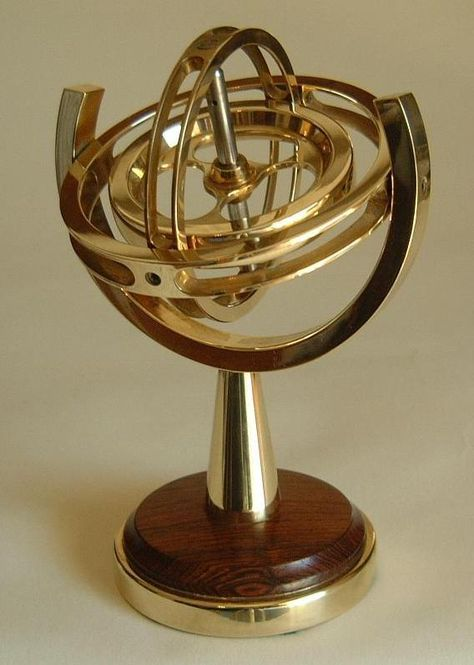
\includegraphics[scale=0.3]{giroskop.jpg}}\hspace{25pt}\qquad
  \subfloat[]{\input{figures/chapter_03/bak_eulera.pdf_tex}}
  \caption{Przykład bąków swobodnych a) żyroskop, \cite{CArn}, b) model bąka Eulera}
  \label{fig:Ch1_giro_model}
    \end{figure}

{\red
  W~przypadku rysunków zawierających kilka części można posłużyć się poleceniem \texttt{\textbackslash subfloat} (zobacz rysunek~\ref{fig:Ch1_giro_model}). Gdy rysunek nie mieści się na jednej stronie, można go podzielić tak, jak to zrobiono w~przypadku rysunku~\ref{fig:portret_fazowy_step} -- użyte mechanizmy dostępne są po dodaniu w~preambule dokumentu pakietu \texttt{subfig}.}
\begin{figure}[tp]
  \centering
  \def\svgscale{0.87}\subfloat[]{\input{figures/chapter_04/elipsoida1a.pdf_tex}}
  \def\svgscale{0.87}\subfloat[]{\input{figures/chapter_04/elipsoida1b.pdf_tex}}\\ 
  \def\svgscale{0.85}\subfloat[]{\input{figures/chapter_04/elipsoida1c.pdf_tex}}
  \def\svgscale{0.85}\subfloat[]{\input{figures/chapter_04/elipsoida1d.pdf_tex}}\\ 
  \def\svgscale{0.83}\subfloat[]{\input{figures/chapter_04/elipsoida1e.pdf_tex}}
  \def\svgscale{0.83}\subfloat[]{\input{figures/chapter_04/elipsoida1f.pdf_tex}}\\ 
  \caption{Kolejne etapy powstawania portretu fazowego (cdn.)}
  \label{fig:portret_fazowy_step}
\end{figure}
\begin{figure}
  \centering
  \ContinuedFloat
  \def\svgscale{0.81}\subfloat[]{\input{figures/chapter_04/elipsoida1g.pdf_tex}}
  \def\svgscale{0.81}\subfloat[]{\input{figures/chapter_04/elipsoida1h.pdf_tex}}\\ 
  \def\svgscale{0.77}\subfloat[]{\input{figures/chapter_04/elipsoida1i.pdf_tex}} 
  \caption{Kolejne etapy powstawania portretu fazowego (cd.)}
\end{figure}

\noindent
[\ldots]

\noindent
Ilustracja opisanej konstrukcji została przedstawiona na rysunku \ref{fig:efekt_poten}. Gdy wykres energii całkowitej nie przecina wykresu $U(\beta)$ oznacza to, że układ taki jest nierealizowany fizycznie jako bąk -- posiada ujemną energię kinetyczną.
\begin{figure}[tp]
    \centering
    \def\svgscale{0.8}
    \input{figures/chapter_04/efektywny_pot.pdf_tex}
    \caption{Wykres efektywnego potencjału}
    \label{fig:efekt_poten}
\end{figure}

\noindent
[\ldots]

\noindent
Gdy $u_L$ zmniejsza się zaczyna formować pętle (rysunek \ref{fig:ul5}).
\begin{figure}[tp]
    \centering
    \subfloat{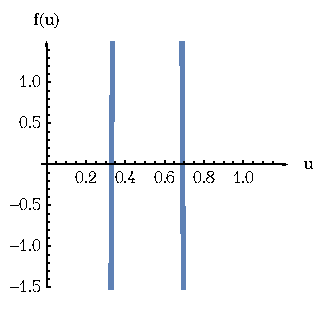
\includegraphics[scale=0.86,valign=m]{figures/chapter_05/ul5_fu.pdf}}
    \subfloat{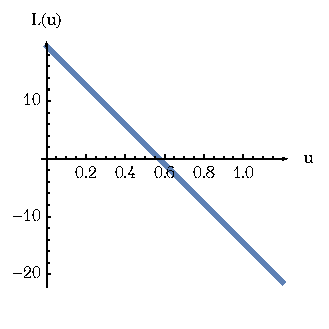
\includegraphics[scale=0.86,valign=m]{figures/chapter_05/ul5_lu.pdf}}
    \subfloat{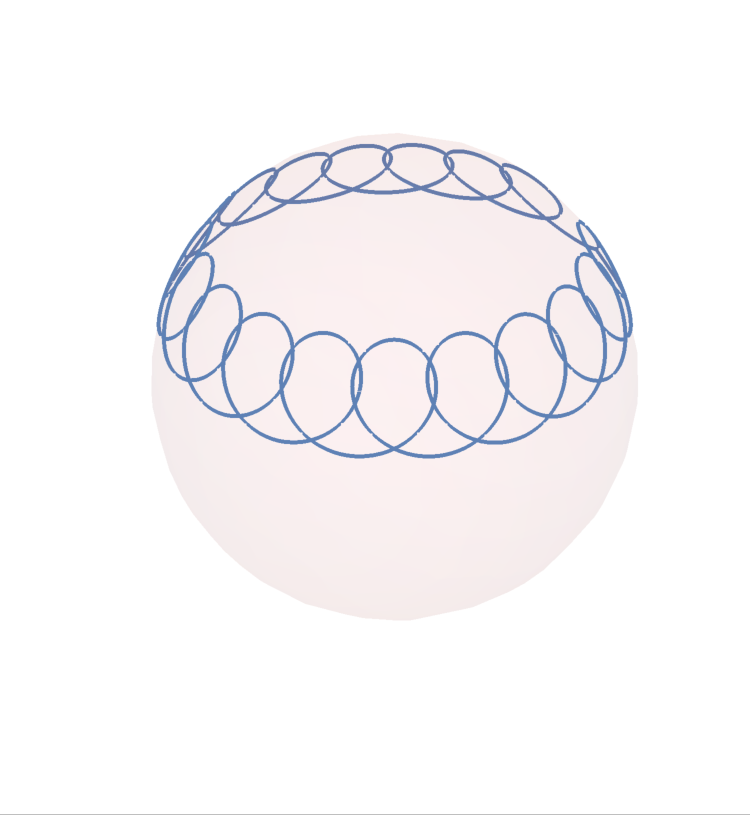
\includegraphics[scale=0.61, trim={1cm 2.5cm 1cm 2.5cm},clip,valign=m]{figures/chapter_05/ul5_trace.pdf}}
    \caption{Przebieg dla $u_1 < u_L < u_2$, $a=114.991$}
    \label{fig:ul5}
\end{figure}

{\red
  Powyższe dwa przykłady (rysunki~\ref{fig:efekt_poten} i~\ref{fig:ul5}) pokazują sposób dołączania wykresów pochodzących z~Inkscape'a i~programu potrafiącego zapisać je w~formacie pdf (Matlab, Mathematica).}

\noindent
[\ldots]

{\red

\section{Inne sprawy}

\subsection{Wykresy, schematy, diagramy, czyli sprawa \texttt{Svg}a i~Ti{\it k}Za}

W~przypadku wykresów i~innych plików, które zostały zapisane w~formacie \texttt{svg} można je dołączyć tak, jak pokazano na rysunku~\ref{fig:svg_input}, na którym to umieszczono wykres wyprodukowany w~środowisku MatLab. 
\begin{figure}[tp]
      \centering
    %\includesvg[scale=0.5, pretex=\scriptsize]{figures/chapter_02/e1_plot_1}
                                          %%w~starszych wersjach pakietu svg nie ma opcji scale :(
    \includesvg[width=0.6\textwidth, pretex=\scriptsize]{e1_plot_1}
    \renewcommand{\figurename}{\red Rysunek}%
    \caption[Wykres uchybu regulacji\ldots]{\red Wykres uchybu regulacji\ldots}
    \label{fig:svg_input}
\end{figure}
Nieco więcej na temat plików \texttt{svg} jest napisane w~komentarzu do rysunku~\ref{fig:transf_se3} na stronie~\pageref{fig:transf_se3}. Alternatywnie wykres można sporządzić korzystając z~pakietu \texttt{pgfplots} \cite{pgfplots} bazującego na języku Ti{\it k}Z. Przykład zaprezentowano na rysunku~\ref{tikz_wykres}.}
\begin{figure}[tp]
  \centering
  \scalebox{0.85}{
    \begin{tikzpicture}
    \begin{axis}[
        title=Kwadratowo,
        xlabel={$x$},
        ylabel={$y$},
      ]
      \addplot table[x expr=\coordindex,y index=0] {figures/chapter_03/data_raw.dat};
    \end{axis}
  \end{tikzpicture}\hspace{5mm}
  \begin{tikzpicture}
    \begin{axis}[
        title=Mój przebieg,
        xlabel={$t$},
        ylabel={$y(t)$},
        grid=major,
      ]
      \addplot [green] table {figures/chapter_03/out.dat};
    \end{axis}
  \end{tikzpicture}}
  \renewcommand{\figurename}{\red Rysunek}%
  \caption[Przykład wizualizacji danych z~pliku]{\red Przykład wizualizacji danych z~pliku}
  \label{tikz_wykres}
\end{figure}

{\red
Jeśli mamy potrzebę przedstawienia prostego schematu blokowego, to może najprościej przygotować go opisując we wspomnianym w~podrozdziale~\ref{narzedzia} języku Ti{\it k}Z, którego tak czy inaczej i~tak warto trochę liznąć. Na rysunkach~\ref{tikz_blok}, \ref{fig:dynamic_lin_diagram} przedstawiono przykłady: pierwszy, prosty, umieszczony w~treści dokumentu i~drugi, bardziej rozbudowany, z~ukazaniem sposobu dołączania z~pliku zewnętrznego\footnote{\red Autor drugiego diagramu bazował na przykładzie \cite{schem_blokowy} i~korzystał z~funkcji \texttt{let} pakietu \texttt{calc}. Po czasie twierdzi, że do przygotowania tak rozbudowanego rysunku użyłby jednak Inkscape'a lub podobnego narzędzia graficznego~\smiley{} Co też w~tym poradniku uczyniono. Po prostu czytaj cierpliwie dalej~\smiley}.}
% zamiast odwołania do rysunku 2.1 wykonać rysunek 3.8 w~Inkscape'ie ale też w~Dia'i
% https://lightonphiri.org/blog/latex-consistent-diagrams-using-dia
%https://en.wikibooks.org/wiki/LaTeX/PGF/TikZ
\begin{figure}[tp]
  \centering
  \scalebox{0.85}{\begin{tikzpicture}[auto, node distance=3.7cm, >=latex]
    
    \node [block] (trajectory) {\makecell{Generator\\trajektorii}};
    \node [sum, right of=trajectory] (sum) {};
    \node [block, right of=sum] (controller) {\makecell{Regulator\\PD}};
    \node [block, right of=controller] (edda) {\makecell{Model\\manipulatora\\EDDA}};
    \node [output, right of=edda] (output) {};
    
    
    \draw [->] (trajectory) -- node {$\mathbf{q_d, \dot{q}_{d}}$} (sum);
    \draw [->] (sum) -- node {$\mathbf{e, \dot{e}}$} (controller);
    \draw [->] (controller) -- node [name=u] {$\mathbf{u}$}(edda);
    \node [output, below of=u, node distance=2cm] (tmp) {};
    
    \draw [->] (edda) -- node [name=y] {$\mathbf{q,\dot{q}}$} (output);
    \draw [->] (y) |- (tmp) -| node[pos=0.99] {$-$} node [near end] {} (sum);
    
      \end{tikzpicture}}
  \renewcommand{\figurename}{\red Rysunek}%
  \caption[Schemat symulowanego układu sterowania dla algorytmu Qu-Dorseya]{\red Schemat symulowanego układu sterowania dla algorytmu Qu-Dorseya}
  \label{tikz_blok}
\end{figure}
\begin{figure}[tp]
  \centering
  \includestandalone[width=0.9\textwidth]{./figures/chapter_02/dynamic-lin}%
  \renewcommand{\figurename}{\red Rysunek}%
  \caption[Dynamic state feedback linearisation \cite{jedrzej}]{\red Dynamic state feedback linearisation \cite{jedrzej}}
    \label{fig:dynamic_lin_diagram}
\end{figure}
{\red Przy opracowywaniu tego typu rysunków można wspomóc się graficznym interfejsem do Ti{\it k}Za o~nazwie TikZiT \cite{tikzit} lub po prostu skorzystać z~Inkscape'a czy podobnego narzędzia, jak opisano to w~punkcie~\ref{grafika_narzedzia} podrozdziału~\ref{narzedzia}. Tutaj, dla przykładu, na rysunku~\ref{fig:dynamic_lin_diagram_ink} pokazano ten sam diagram co na rysunku~\ref{fig:dynamic_lin_diagram} przygotowany właśnie z~użyciem Inkscape'a\footnote{\red Diagramy nie są idealnie identyczne -- niestety opracowując w~Inkscape'ie grafikę w~której zostaną użyte te same czcionki co w~tekście wszystkie napisy trzeba pozycjonować ręcznie, co w~przypadku Ti{\it k}Za dzięki użyciu pakietu \texttt{calc} odbywa się automatycznie\footnotemark. Ci co zajrzeli do pliku źródłowego \texttt{dynamic-lin\_ink.svg}\footnotemark{} wiedzą o~co chodzi \smiley{}  Inny przykład inkscape'owego rysunku pokazano na stronie~\pageref{fig:transf_se3}.}\addtocounter{footnote}{-1}\footnotetext{\red No prawie zawsze \smiley}\addtocounter{footnote}{1}\footnotetext{\red Oczywiście przy użyciu programu Inkscape \smiley}.
\begin{figure} [tp]
  \centering%
  \scalebox{1.0}{\def\svgwidth{0.9\textwidth}
    \input{figures/chapter_02/dynamic-lin_ink.pdf_tex}}
  \renewcommand{\figurename}{\red Rysunek}%
  \caption[Dynamic state feedback linearisation from Inkscape \cite{jedrzej}]{\red Dynamic state feedback linearisation from Inkscape \cite{jedrzej}}
    \label{fig:dynamic_lin_diagram_ink}
\end{figure}
Podobnie można postąpić, gdy potrzebujemy przygotować jakiś diagram przepływu danych czy też diagram algorytmu, choć tu prymarnym wyborem może się okazać program Dia\todo{Dodać przykład w~Dia \cite{dia_fonty}} \cite{dia,dia_wiki}.

  
\subsection{Kod źródłowy, pseudokod, czyli trudna sprawa}

W~zasadzie wydaje się, że wystarczyłoby napisać, iż do umieszczania w~dokumentach kodu źródłowego służy pakiet \texttt{listings}. Jednakże w~podstawowej wersji zapewniane przez niego formatowanie jest bardzo ubogie, co zazwyczaj prowadzi do potrzeby jego konfigurowania. Przykłady jak to zrobić można znaleźć na stronie \cite{list_wiki} czy w~dokumentach opisujących użycie tego pakietu. Alternatywę dla pakietu \texttt{listings} stanowi ostatnio coraz popularniejszy pakiet \texttt{minted}\footnote{\red Jednakże korzystanie z~tego pakietu wymaga zainstalowania kompilatora Phytona oraz systemu podświetlania składni Pygments, zaś sam kompilator pdflatecha musi być wywoływany z~dodatkową opcją \texttt{--shell-escape}.}, z~którego skorzystamy w~poniższych przykładach. Zanim jednak pojawią się przykłady, kilka słów wyjaśnienia, czemu sprawa jest trudna.

Zasadniczo, trudno jest wskazać jedno, uniwersalne rozwiązanie wygodne do przytaczania fragmentów programów, algorytmów zapisanych w~pseudokodzie. Mo\-żna je chociażby umieszczać bezpośrednio w~tekście, jako obiekty pływające w~postaci rysunków, czy też jako obiekty pływające utworzone niezależnie od rysunków. Co lepiej zapewne zależy od tego, czy w~pracy będziemy mieli mnóstwo takich wydruków, czy tylko kilka, czy będą długie, czy krótkie, czy towarzyszyć im będzie dużo tekstu, czy niewiele. Sprawa dodatkowo komplikuje się, jeśli nasze wydruki nie będą mieścić się na pojedynczej stronie i~trzeba będzie je umieszczać jako obiekty wielostronicowe. A~do tego trzeba zadbać o~prawidłowe kodowanie narodowych liter diakrytyzowanych, jeśli takowe w~dołączanych wydrukach występują\footnote{\red Nie wszystkie kroje czcionek używane typowo do składu wydruków zawierają inne, niż podstawowe znaki diakrytyczne.}. Tak czy inaczej, by nie mieć z~kodem źródłowym problemów warto rzecz przemyśleć już na początku pracy z~dokumentem, wybrać jedno, dwa środowiska, naszym zdaniem wygodne w~danej sytuacji i~trzymać się przyjętego rozwiązania.

By przytoczyć wydruk programu bezpośrednio w~tekście wystarczy użyć otoczenia \texttt{minted}
  \begin{minted}[bgcolor=OurListingBackground,linenos=true]{c}
    int pow3(int x) {
      return x * x * x;
    }

    int a = 2, b = 3;
    int y = pow3(a) + b;
    int z = a + pow3(y);
  \end{minted}
W~typowych instalacjach takie rozwiązanie pozwala na podświetlanie wydruków z~ponad 300 języków programowania, na używanie styli\footnote{\red polecenie \texttt{\textbackslash usemintedstyle} -- odkomentuj w~preambule tego dokumentu, by zobaczyć efekt} a~także umieszczanie odpowiednio podświetlonych fragmentów kodu \mintinline{python}{print(x**2)} w~tekście.

Jeśli decydujemy się na umieszczanie wydruków w~sposób wystawiony, możemy do tego celu użyć po prostu otoczenia \texttt{figure}\footnote{\red Co wydaje się rozsądne, gdy w~naszym tekście jest niedużo tak sformatowanych wydruków -- będą one numerowane jednolicie z~rysunkami i~będziemy mówić po prostu, że dany wydruk jest umieszczony na rysunku~\ref{rys:wyd}.}
\begin{figure}[tp]
    \begin{minted}[frame=single,framesep=10pt,fontsize=\scriptsize]{c}
void full_2_cse_static_lin_eta(float eta[5], const float u[5], const float q[9])
{
    float x0 = q[4];
    float x1 = q[2];
    float x2 = sinf(x1);
    float x3 = 1.0F/R;
    float x4 = u[0]*x3;
    float x5 = cosf(x1);
    float x6 = u[1]*x3;
    float x7 = q[3];
    float x8 = 1.0F/cosf(x7);
    float x9 = x4*x5;

    eta[0] = -u[3]*sinf(x0) + x2*x4 - x5*x6;
    eta[1] = u[3]*cosf(x0)*tanf(x7) + x10*x8 + x8*x9;
    eta[2] = u[3];
}
    \end{minted}
  \renewcommand{\figurename}{\red Rysunek}%
  \caption[Przykładowy wydruk umieszczony na rysunku]{\red Przykładowy wydruk umieszczony na rysunku}
    \label{rys:wyd}
\end{figure}
lub dostarczonego przez pakiet \texttt{minted} otoczenia \texttt{listing}, co spowoduje, że wydruki programów będą numerowane niezależnie i~nazywane wydrukami, jak ten pokazany na wydruku~\ref{lst:example}.
\begin{listing}[tp]
    \begin{minted}[frame=single,framesep=10pt,fontsize=\scriptsize]{c}
void full_2_cse_static_lin_eta(float eta[5], const float u[5], const float q[9])
{
    float x0 = q[4];
    float x1 = q[2];
    float x2 = sinf(x1);
    float x3 = 1.0F/R;
    float x4 = u[0]*x3;
    float x5 = cosf(x1);
    float x6 = u[1]*x3;
    float x7 = q[3];
    float x8 = 1.0F/cosf(x7);
    float x9 = x4*x5;

    eta[0] = -u[3]*sinf(x0) + x2*x4 - x5*x6;
    eta[1] = u[3]*cosf(x0)*tanf(x7) + x10*x8 + x8*x9;
    eta[2] = u[3];
}
    \end{minted}
\SetupFloatingEnvironment{listing}{name=\red Wydruk}
\caption{\red Przykładowy kod programu}
\label{lst:example}
\end{listing}
Należy jednak pamiętać, że takie formatowanie ogranicza wielkość kodu do pojedynczej strony.

By dowiedzieć się więcej na temat tego, jak automatycznie łamać długie linie w~kodzie programu, jak łamać kod pomiędzy kolejnymi stronami i~tym podobnych spraw, wystarczy zajrzeć do dokumentacji pakietu \texttt{minted} \cite{minted}.}

\chapter{Podsumowanie}

Celem pracy było zapoznanie z opisem dynamiki ruchu bąków ciężkich oraz przygotowanie systemu symulacji, pozwalającego na badanie zachowania układu w~czasie, co zostało zrealizowane. W pracy przytoczono podstawowy aparat matematyczny niezbędny do\ldots{} Podano w niej opis ruchu ciała sztywnego\ldots{} Pokazano równoznaczność opisu\ldots{} Dla kompletności krótko scharakteryzowano\ldots

Przedstawiony w pracy ogólny opis dynamiki ruchu bąka został uzyskany z wykorzystaniem\ldots{} Opis zawarty w pracy umożliwia porównanie\ldots{} Matematyczne modele zostały poparte ich ilustracjami oraz, o ile było to możliwe, przykładem fizycznym.

W pracy kolejno przeprowadzono analizę jakościową równań\ldots{} W celu uzupełnienia opisu analitycznego badaniami symulacyjnymi opracowano program pozwalający na\ldots{}

{\red
  W~podsumowaniu należy przede wszystkim napisać, co było celem pracy i~w~jaki sposób został on zrealizowany. A~dalej, co dokładnie w~jej ramach zostało wykonane, jak zostało to przedstawione, na co przedstawiony materiał pozwala, co z~niego wynika. Podsumowanie powinno także zasadniczo zawierać wyodrębnioną specyfikację oryginalnego wkładu autora do pracy.}

Pomimo swojej prostoty bądź nawet prymitywności bąk potrafi zaciekawić, a~nawet zainspirować rozmaitością ruchów oraz ich ewolucji. W trakcie przeglądu literatury nie napotkano na obiekt będący uogólnieniem bąka, podobnym do uogólnienia, jakim jest podwójne wahadło dla wahadła, które może stanowić źródło interesujących zachowań, również z punktu widzenia teorii układów chaotycznych. Bąki pełnią nie tylko rolę edukacyjną, jako wprowadzenie w arkana mechaniki analitycznej, ale również rozrywkową, a nawet estetyczną. Mamy nadzieję, że przybliżenie czytelnikowi tematyki bąków zaowocuje zaopatrzeniem się w jednego z nich, puszczeniem go i medytacją nad jedną z wielu jego twarzy.

{\red
  Dalsza część podsumowania powinna zawierać wnioski płynące z~pracy, a~także wskazywać potencjalne kierunki dalszych prac\footnote{\red Czego akurat w~tej przykładowej pracy nie uczyniono.}.}


\cleardoublepage
\phantomsection
\addcontentsline{toc}{chapter}{\bibname}
\bibliographystyle{alphapl}
\bibliography{sources/bibliografia}
\markboth{\bibname}{\bibname}   % to niestety nie działa by usunąć MakeUppercase z~nagłówków w~literaturze

%%spis tabel
%\cleardoublepage
%\phantomsection
%\listoftables
%\addcontentsline{toc}{chapter}{\listtablename}
%\markboth{\listtablename}{\listtablename}

%%spis rysunków
\cleardoublepage
\phantomsection
\addcontentsline{toc}{chapter}{\listfigurename}
\listoffigures
\markboth{\listfigurename}{\listfigurename}

\appendix
\chapter{Bąkiem malowane}
\markboth{Bąkiem malowane}{Bąkiem malowane}

Ponieważ niektóre otrzymywane ślady ruchu bąków bywały niezwykle artystyczne i wprawiały nas w zdumienie zdecydowaliśmy się pokazać co ciekawsze ku uciesze czytelnika. Zestaw śladów, który najbardziej przypadł nam do gustu przedstawiono na rysunku \ref{fig:top_life} \cite{Joniak}.
\begin{figure}[tp]
  \centering
  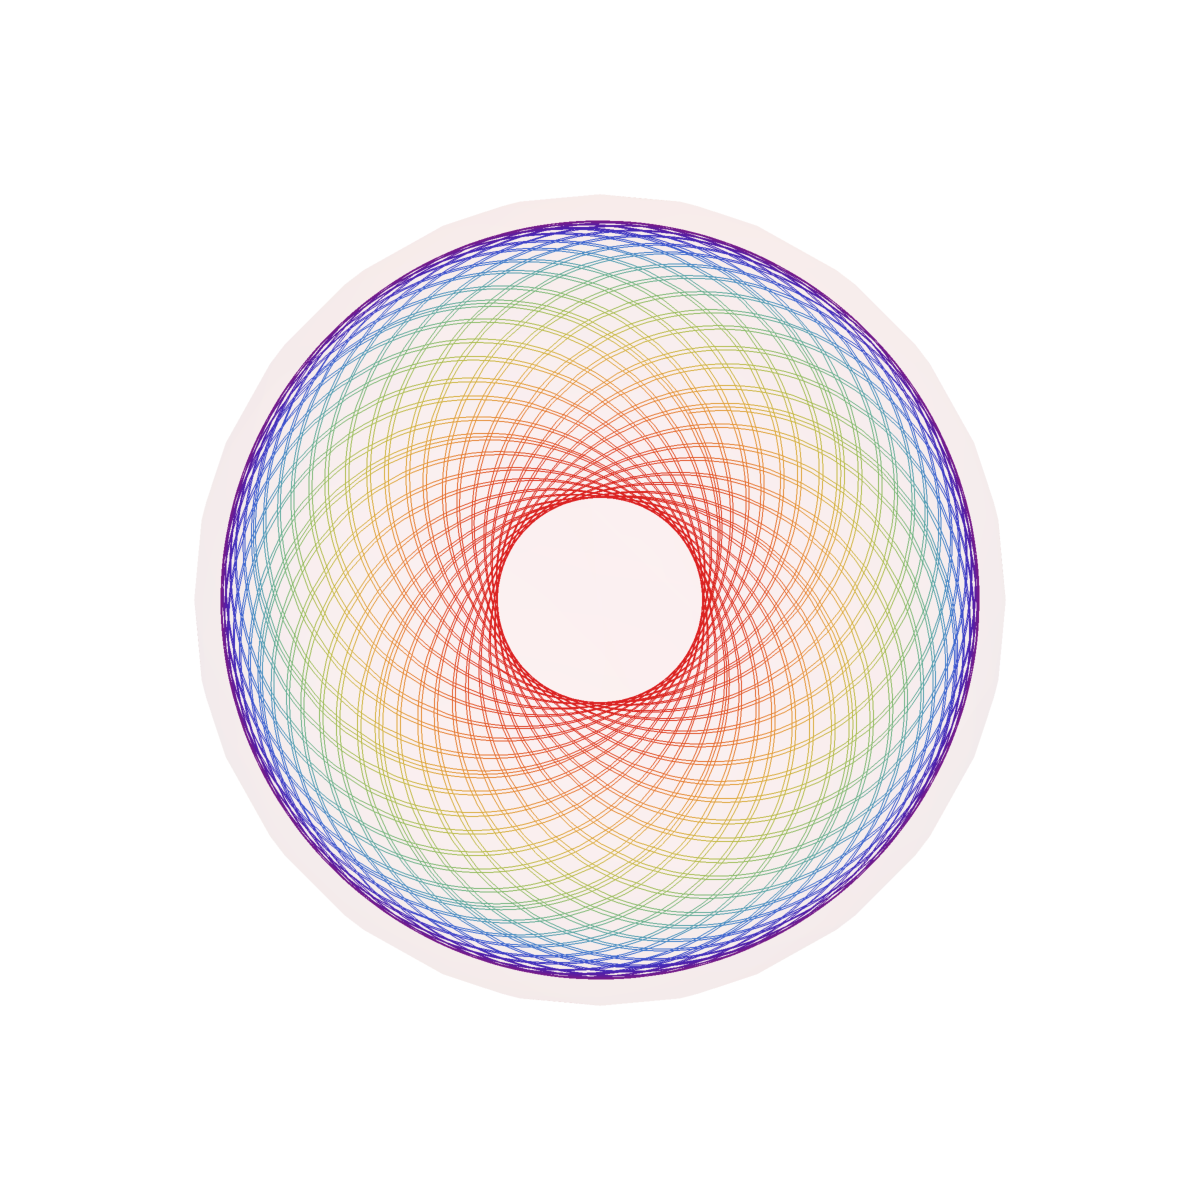
\includegraphics[scale=0.7]{figures/chapter_06/mal2.pdf}
  \caption{Atom}
\end{figure}
%
\begin{figure}[tp]
  \centering
  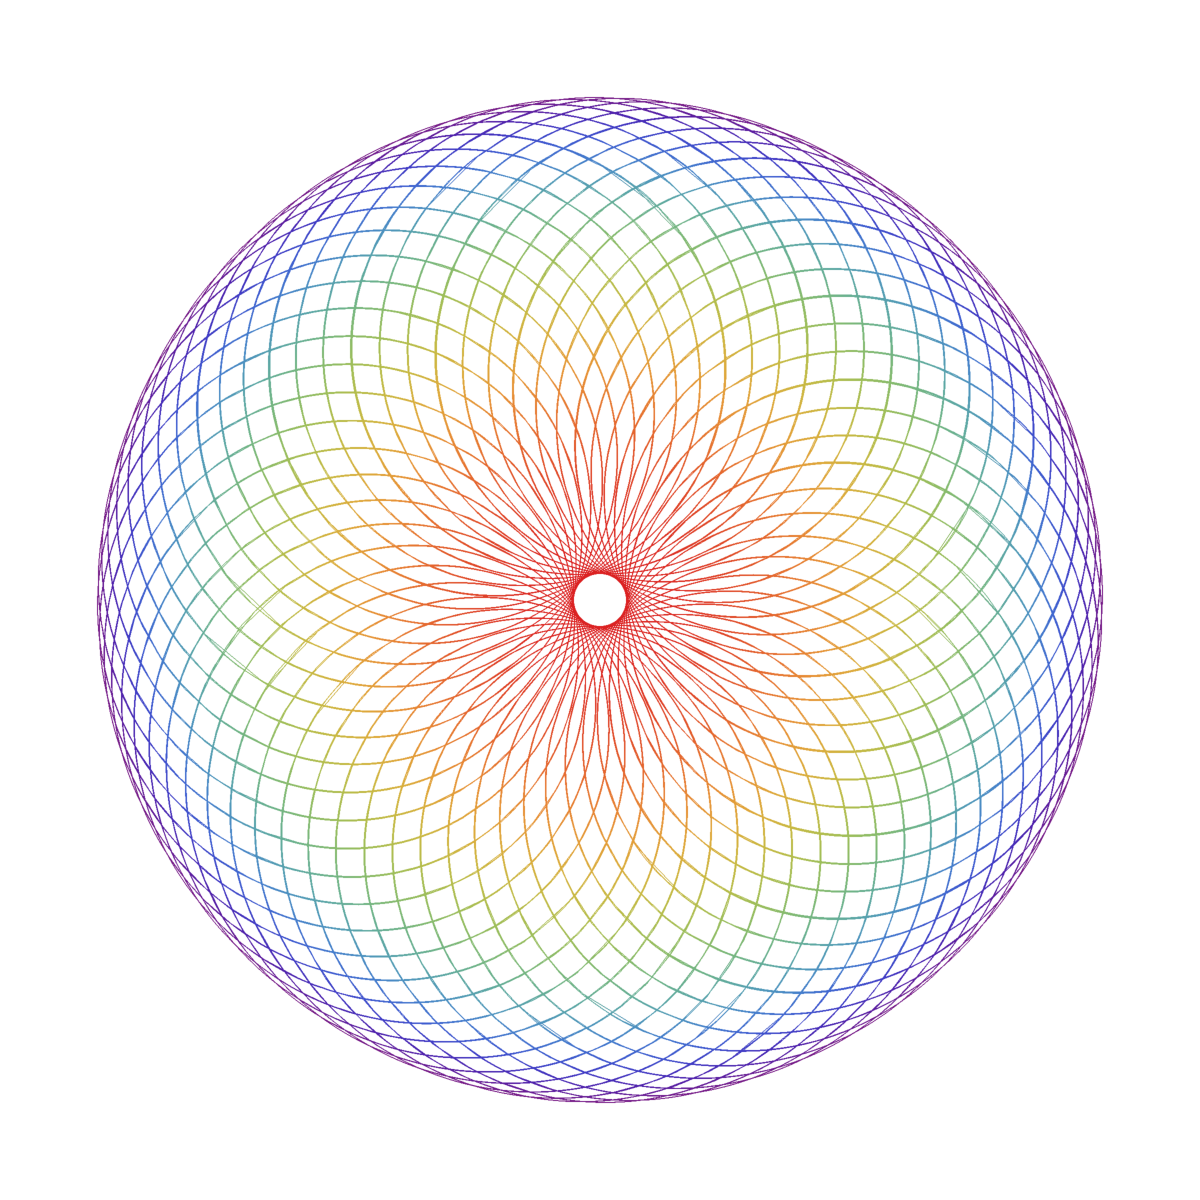
\includegraphics[scale=0.5]{figures/chapter_06/mal4.pdf}
  \caption{Słonecznik}
\end{figure}
%
\begin{figure}[tp]
  \centering
  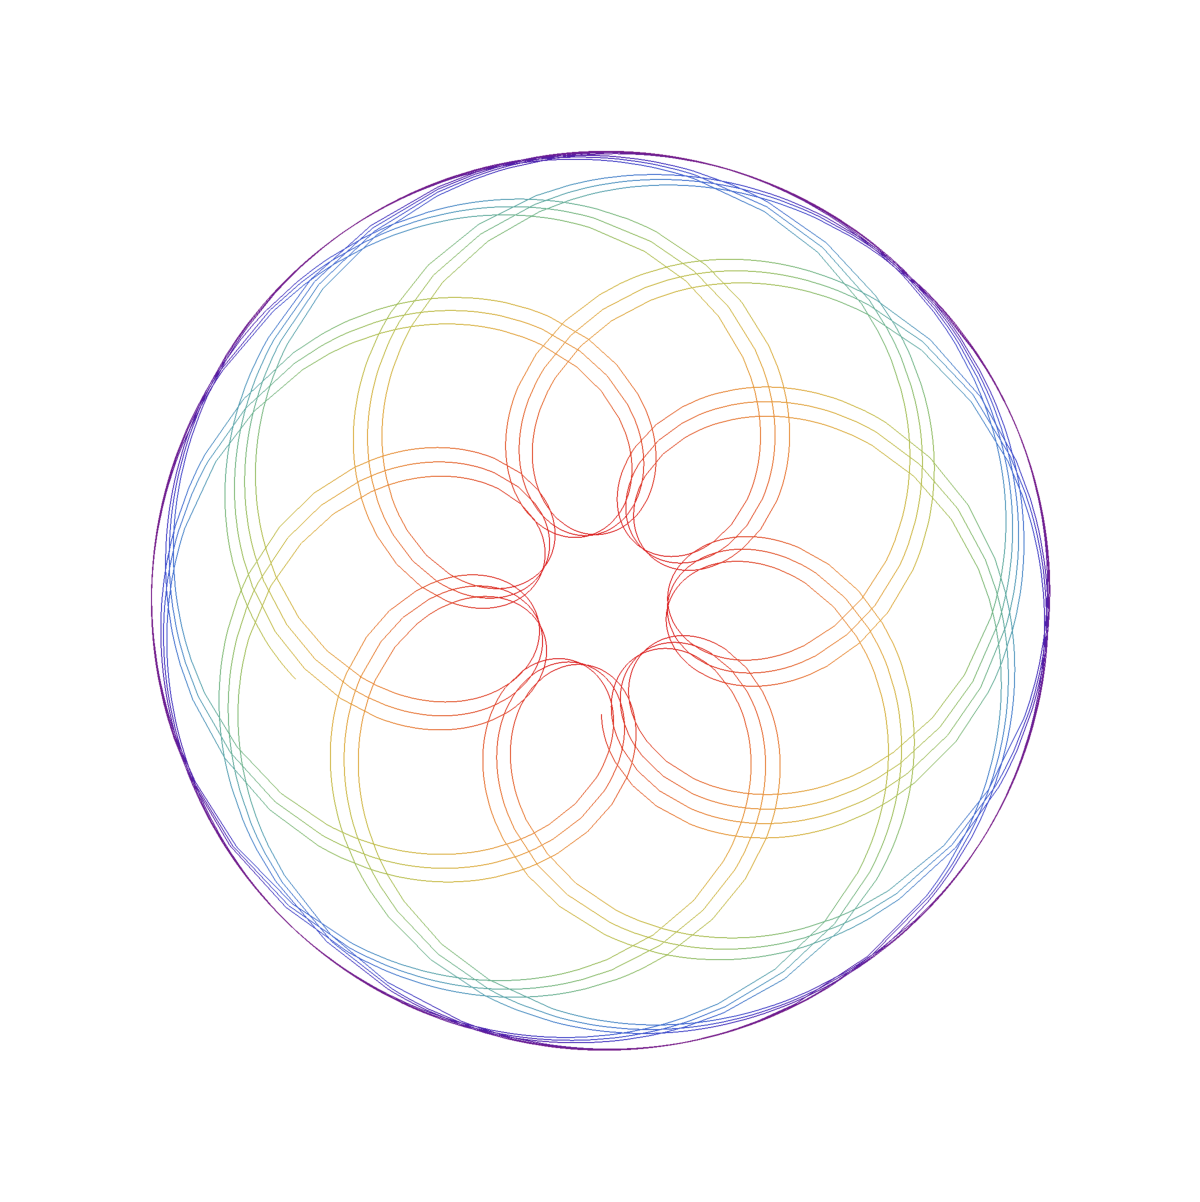
\includegraphics[scale=0.5]{figures/chapter_06/mal5.pdf}
  \caption{Kwiat}
\end{figure}
%
\begin{figure}[tp]
  \centering
  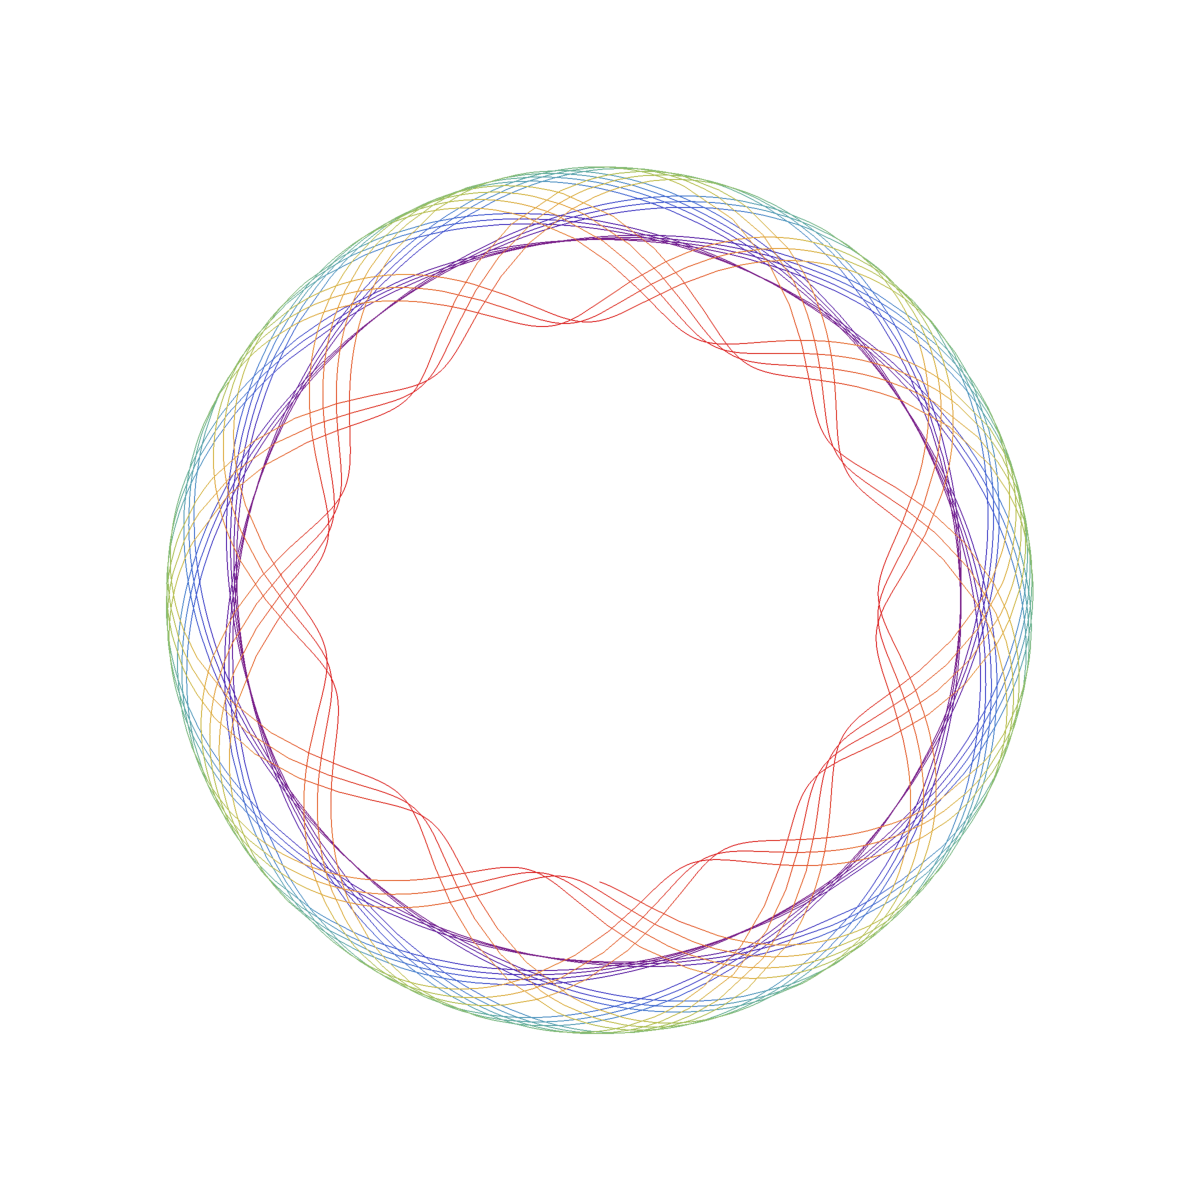
\includegraphics[scale=0.5]{figures/chapter_06/mal8.pdf}
  \caption{Gwiazda}
\end{figure}
%
\begin{figure}[tp]
  \centering
  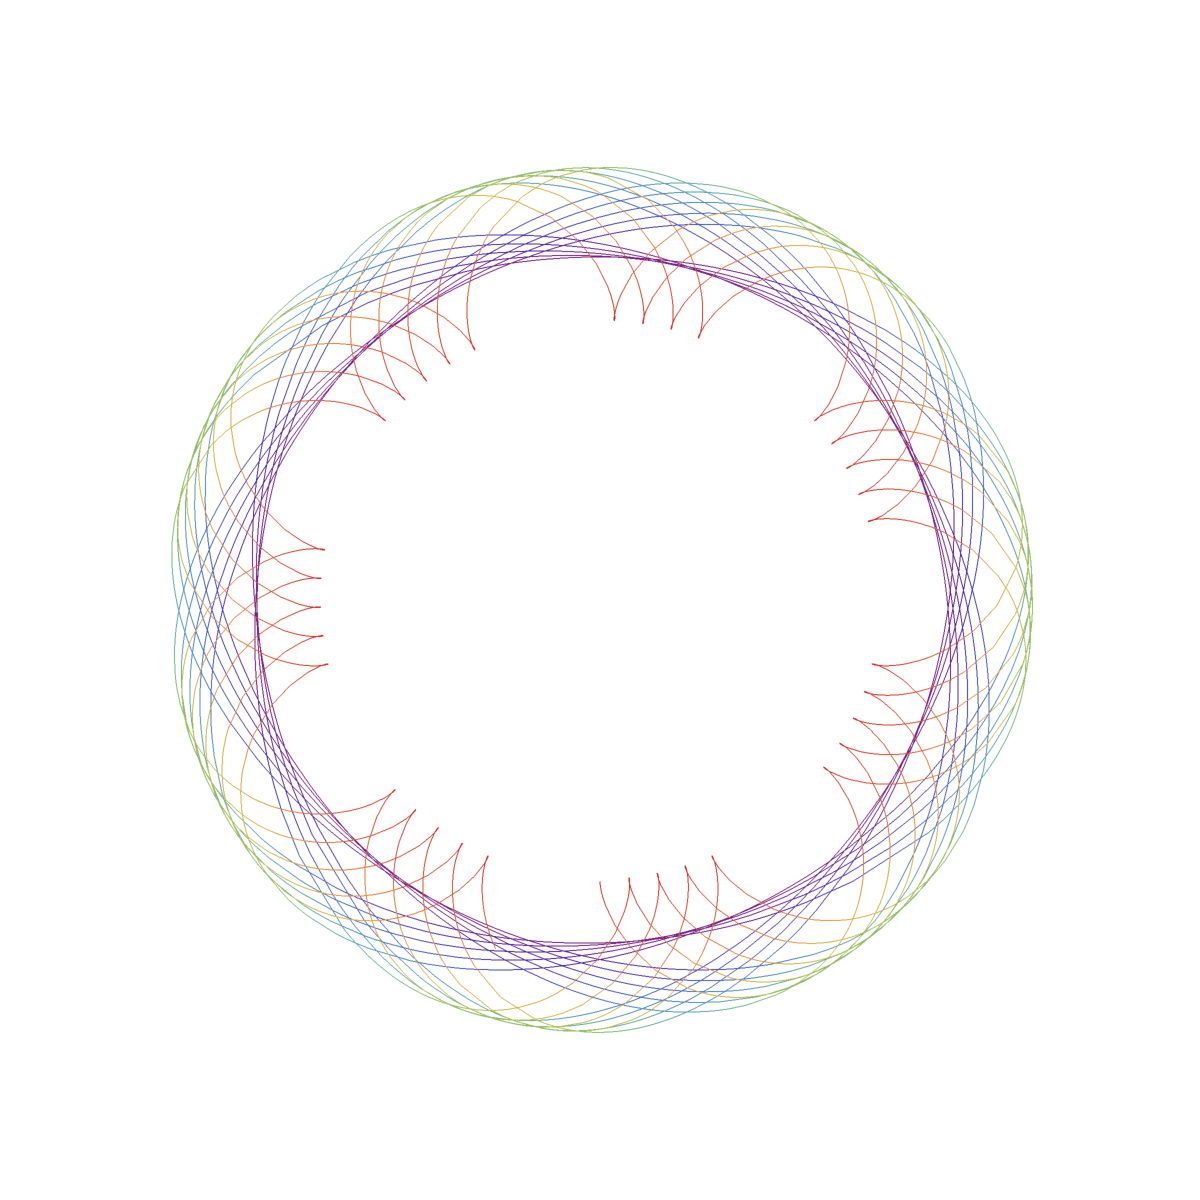
\includegraphics[scale=0.5]{figures/chapter_06/mal7b.pdf}
  \caption{Paszcza}
\end{figure}
%
\begin{figure}[tp]
  \centering
  \subfloat{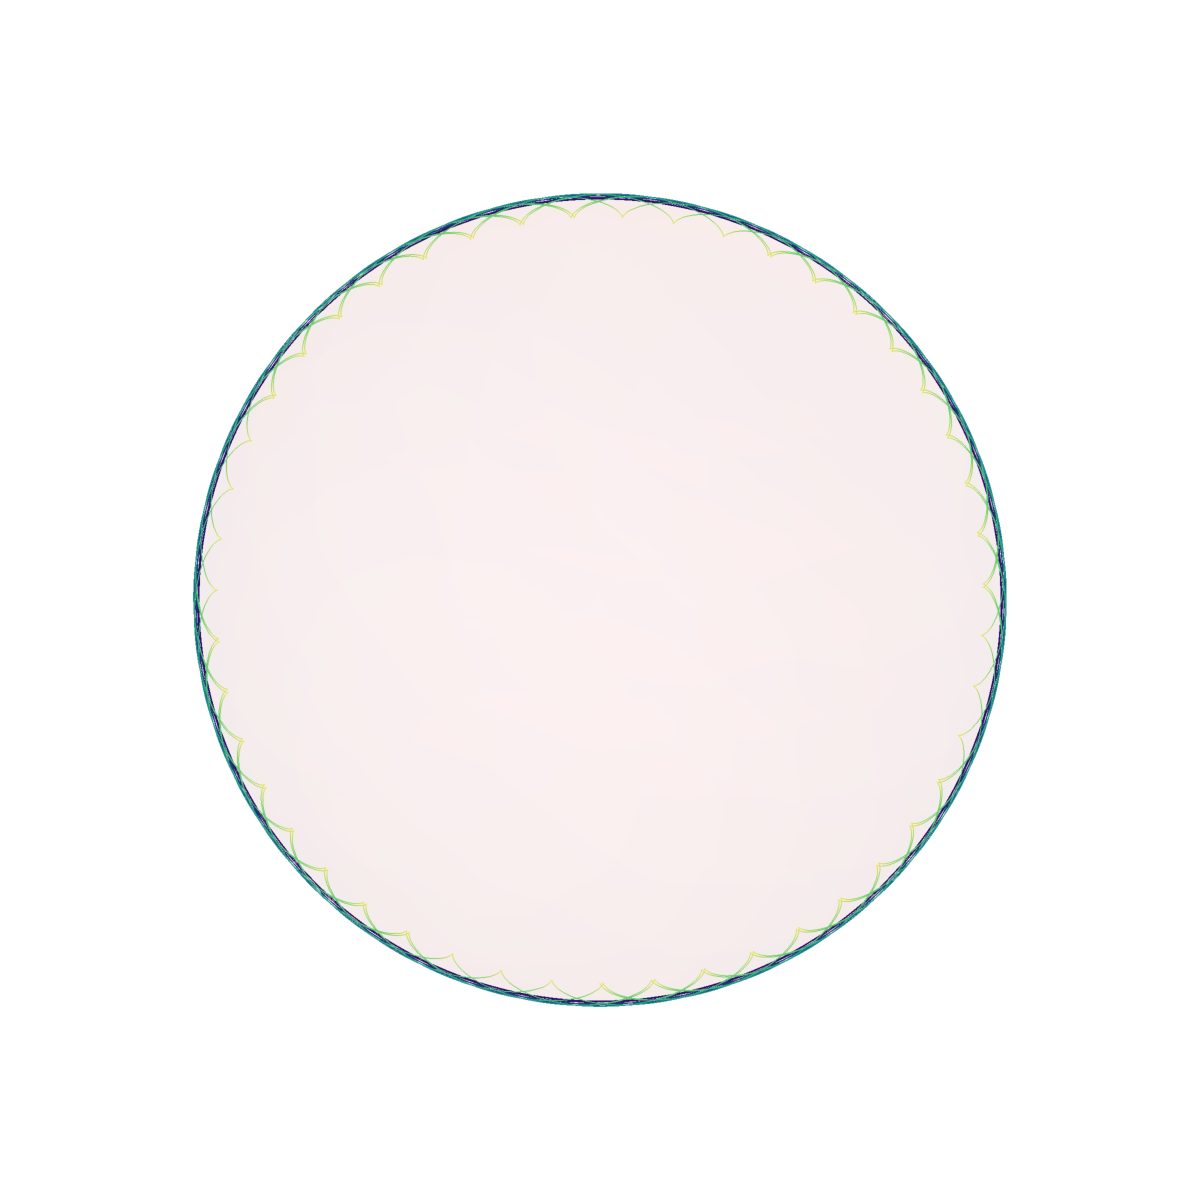
\includegraphics[scale=0.45,trim={2cm 2cm 2cm 2cm}, clip]{figures/chapter_06/malowane_-1.pdf}}
  \subfloat{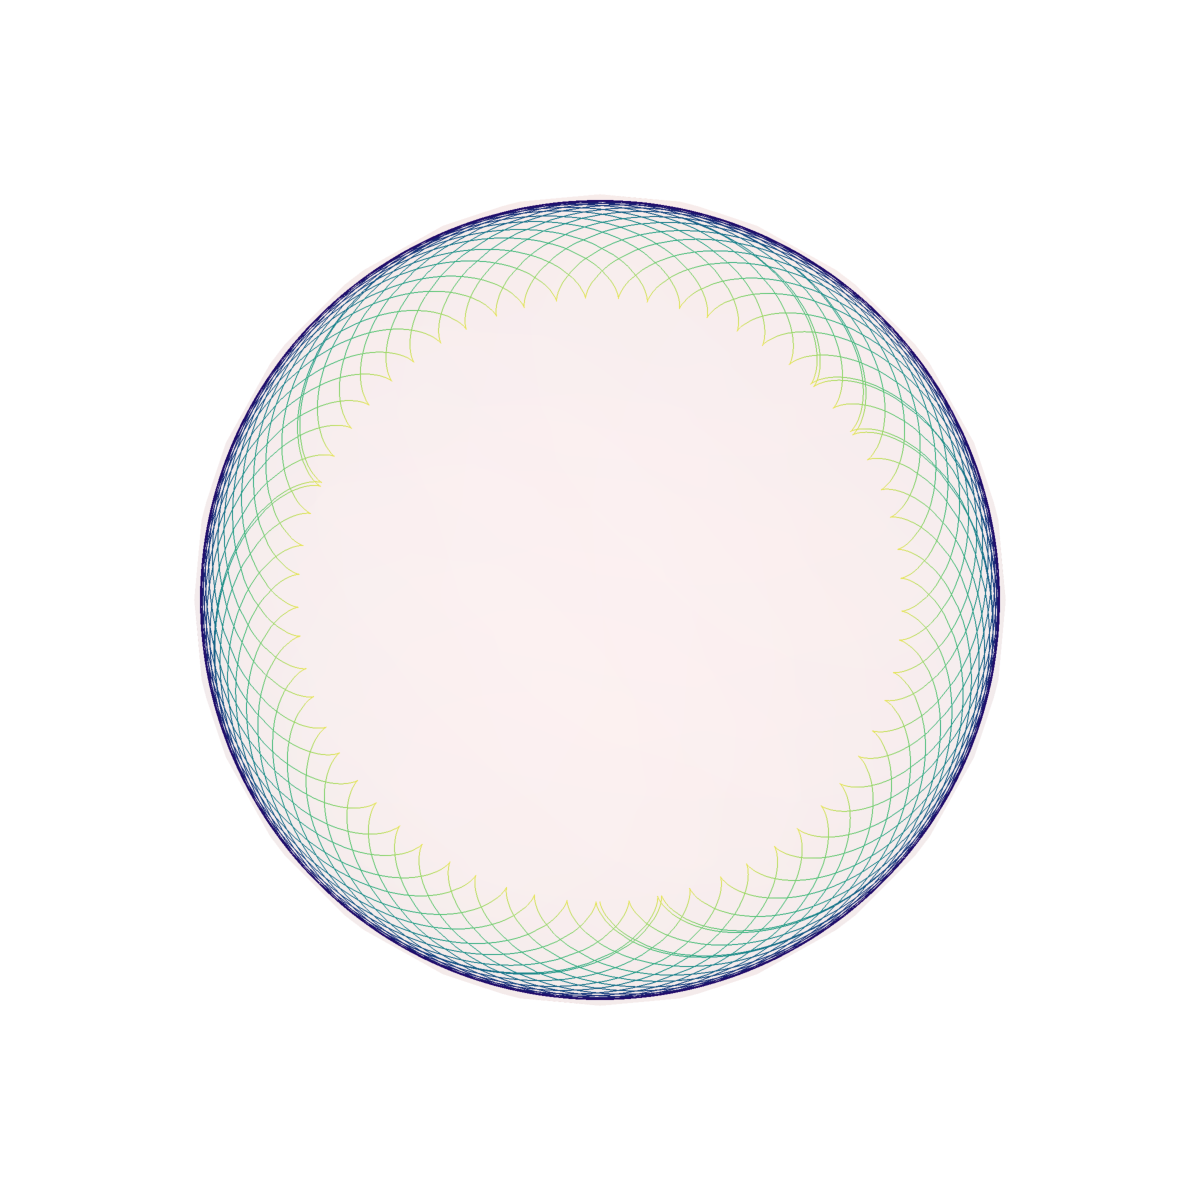
\includegraphics[scale=0.45,trim={2cm 2cm 2cm 2cm}, clip]{figures/chapter_06/malowane_4.pdf}}\\
  \subfloat{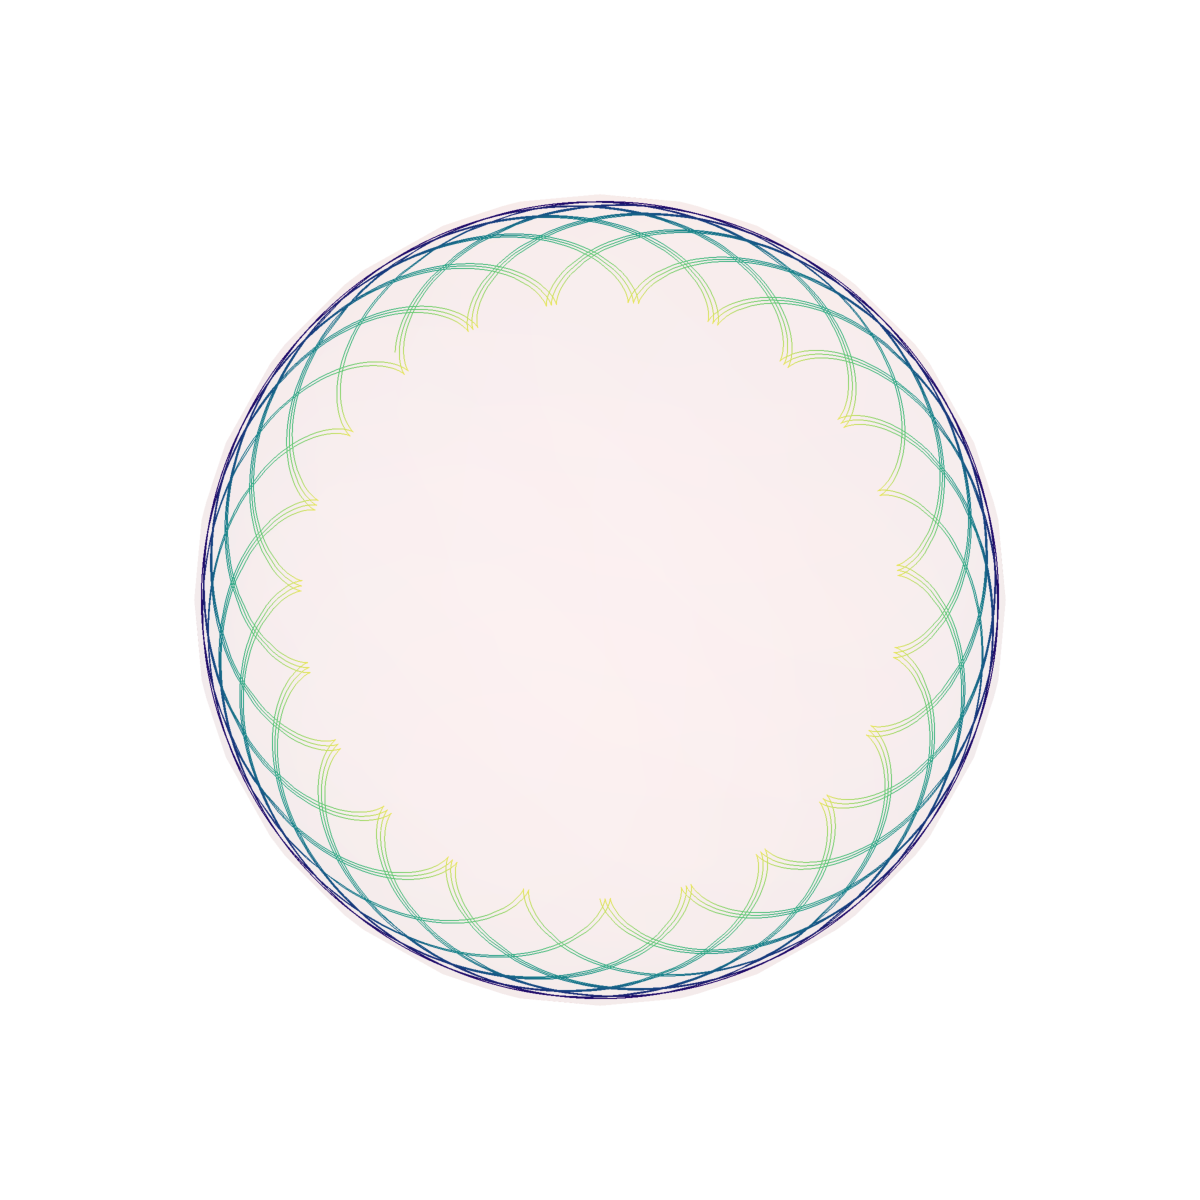
\includegraphics[scale=0.45,trim={2cm 2cm 2cm 2cm}, clip]{figures/chapter_06/malowane_0.pdf}}
  \subfloat{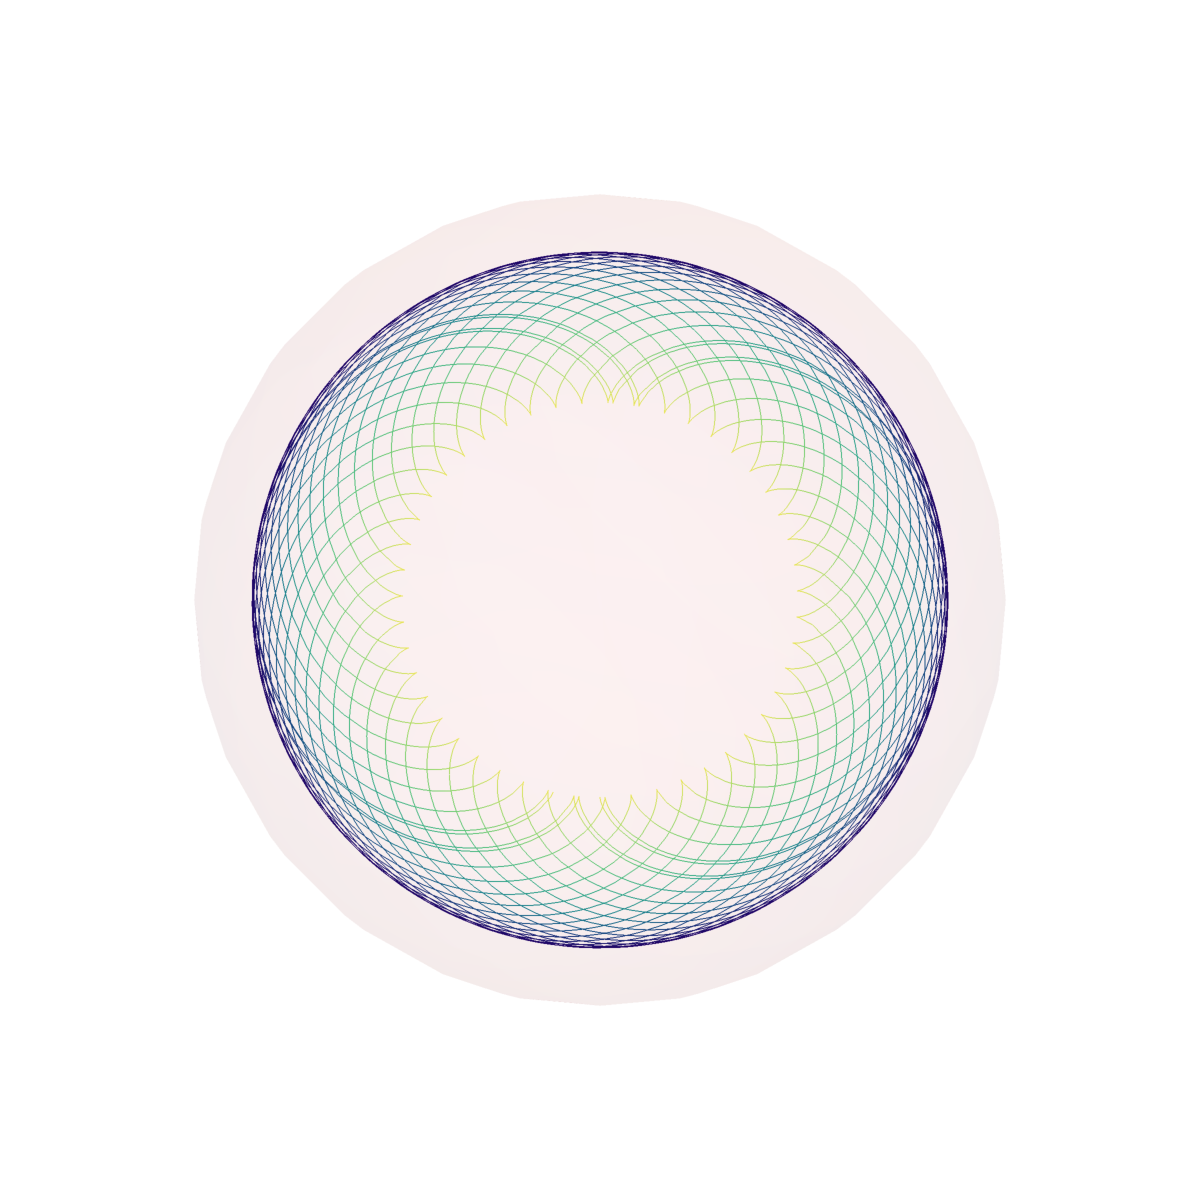
\includegraphics[scale=0.45,trim={2cm 2cm 2cm 2cm}, clip]{figures/chapter_06/malowane_2.pdf}}\\
  \subfloat{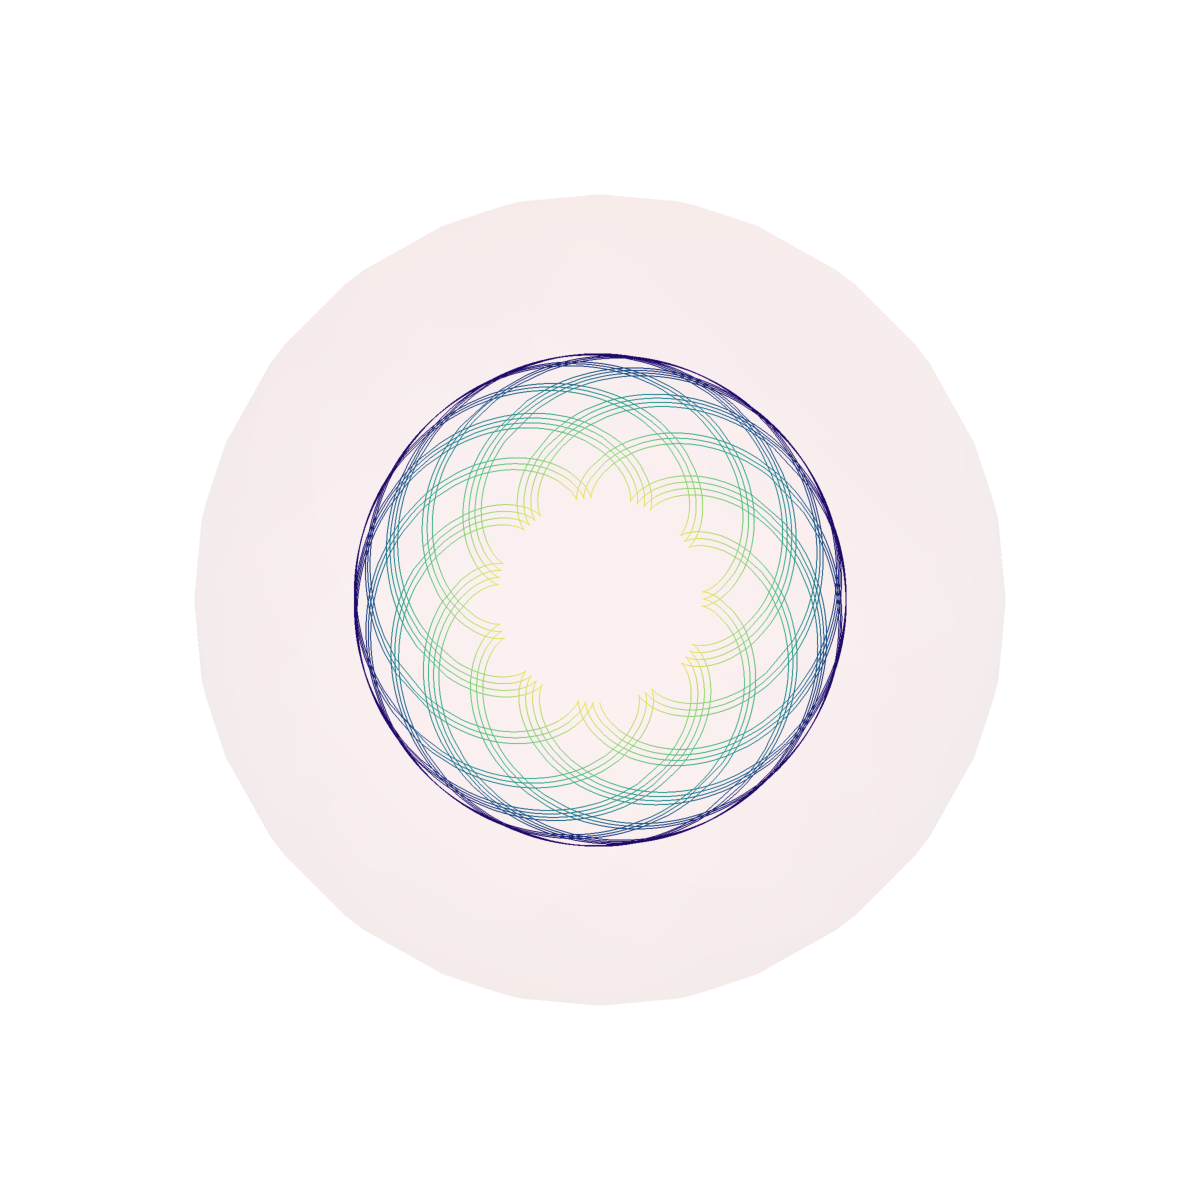
\includegraphics[scale=0.45,trim={2cm 2cm 2cm 2cm}, clip]{figures/chapter_06/malowane_3.pdf}}
  \subfloat{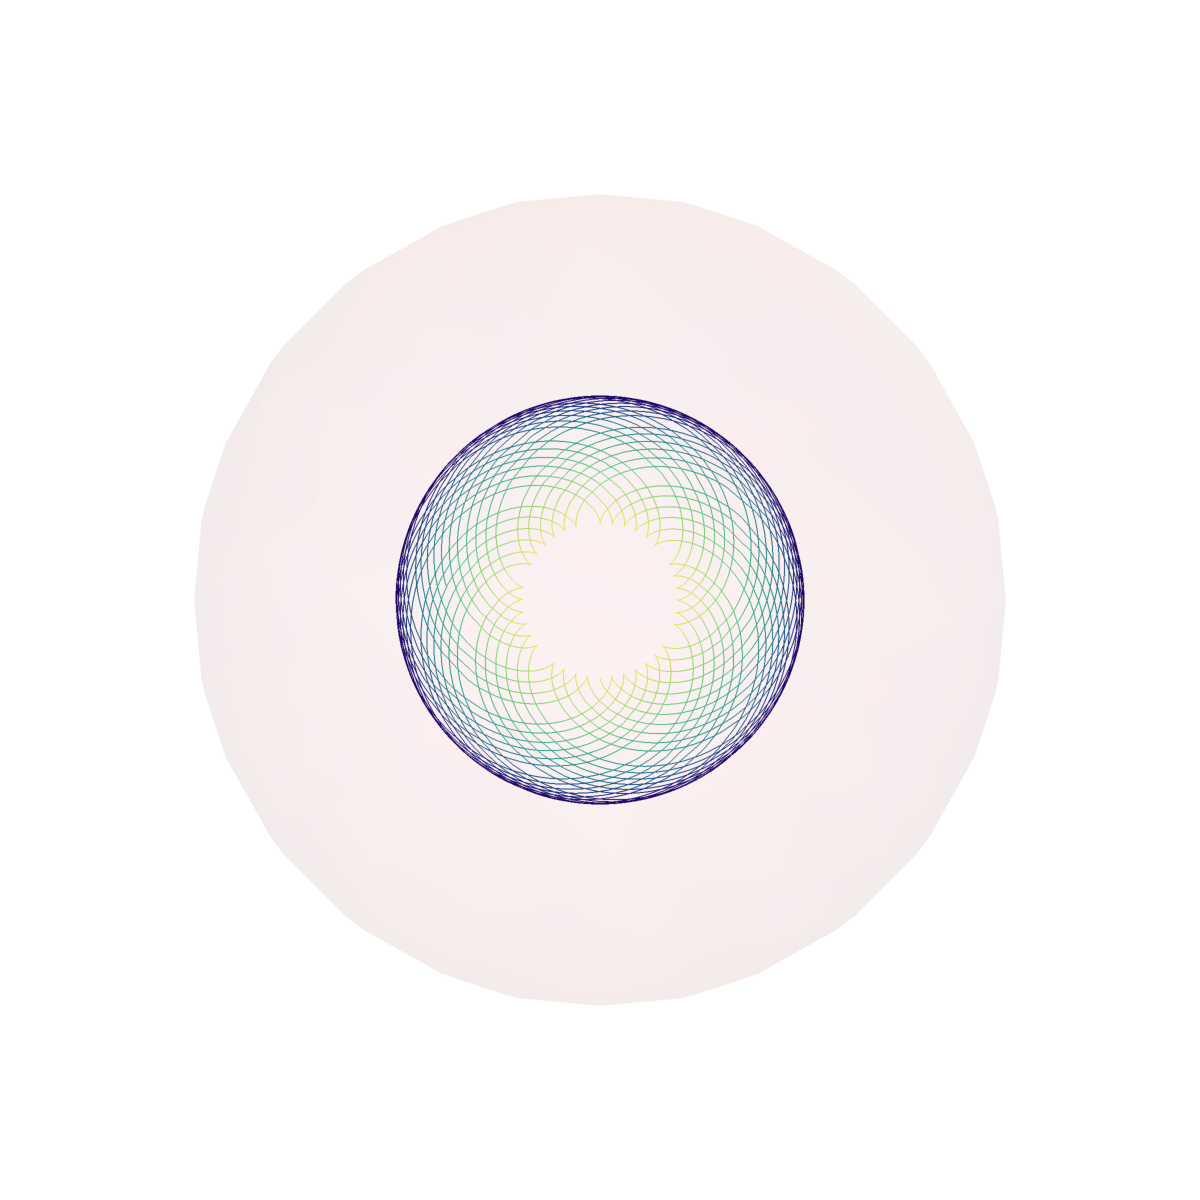
\includegraphics[scale=0.45,trim={2cm 2cm 2cm 2cm}, clip]{figures/chapter_06/malowane_6.pdf}}
  \caption{Życie bąka}
  \label{fig:top_life}
\end{figure}

{\red
  Czasami pojawia się potrzeba umieszczenia w~pracy dodatków. Wówczas
  wystarczy poprzedzić je poleceniem \texttt{\textbackslash appendix}
  i~voilà, mamy co potrzebowaliśmy. Tu można umieszczać rzeczy
  poboczne, kod programu, dowód jakiegoś twierdzenia, w~większej
  liczbie symulacje, wyniki, czy też może jakąś galerię \smiley}


%% lista rzeczy do zrobienia
\listoftodos

\end{document}
